\documentclass{report}
\usepackage{ugentstyle}



\newenvironment{grammarfigure} % Environment that changes the caption name to "Grammatica" for figures
{
	\renewcommand{\figurename}{Grammatica}
	\begin{figure}[h]
}
{
	\end{figure}
	\renewcommand{\figurename}{Figuur}
}


% commando om vraag-antwoord situaties te behandelen
\newcommand{\QA}[2]{
	\noindent\fbox{
		\parbox{\linewidth}{
			\textbf{Q:} #1
			
			\textbf{A:} #2
		}
	}
}


\begin{document}
	\maketitle{Compilers}
	\tableofcontents
	\part{Theorie}
	\chapter{Inleiding}
\section{Compilers}
Voorbeelden van functies die een statische compiler moet bevatten:
	\begin{itemize}
		\item Broncode omzetten in uitvoerbare fouten:
		\begin{itemize}
			\item met dezelfde semantiek
			\item zo snel mogelijk
			\item en/of zo compact, debugbaar, portable, veilig, ... mogelijk
			\item en linkbaar.
		\end{itemize}
		\item Syntaxfouten moeten herkent worden.
	\end{itemize}

\section{Basiswerking compilers}
\begin{figure}[h]
	\centering
	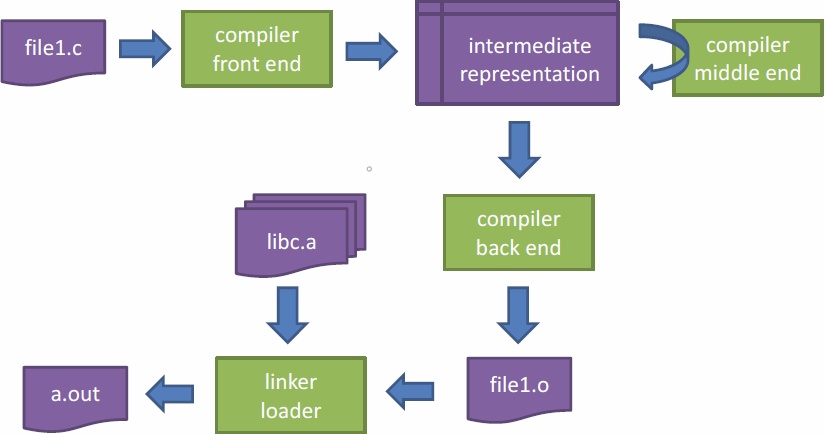
\includegraphics[width=0.5\textwidth]{basiswerking_compilers}
	\caption{De basiswerking van een compiler.} 
	\label{fig:basiswerking_compilers}
\end{figure}
Op figuur \ref{fig:basiswerking_compilers} is de vereenvoudigde basiswerking van een compiler te zien. Een \textbf{C} bestand wordt eerst door de \uline{compiler front end} gestuurd, die het bestand zal omvormen tot een intermediaire representatie. Deze representatie wordt dan door de \uline{compiler back end} gestuurd om zo assembly of objectcode te genereren. De \uline{linker loader} zal deze objectcode samenvoegen met eventuele andere libraries om zo een uitvoerbaar programma te hebben. 

\QA{Waarom wordt de front end en back end opgesplitst?}
{Op die manier is de compiler modulair: Enerzijds moet bij een andere programmeertaal enkel de front end aangepast worden en anderzijds moet bij het wijzigen van de architectuur (de onderliggende processor) enkel de back end aangepast worden.}


\section{Abstract Syntax Tree}
De eerste stap van elke compiler is het omvormen van de broncode naar een \textbf{Abstract Syntax Tree (AST)}. Veronderstel volgende code, en de daarbijhorende AST die te zien zijn op figuur \ref{fig:abstract_syntax_tree}. Elke knoop van een AST stelt een bepaalde geldige operatie voor, die afhankelijk is van de gekozen programmeertaal.
\begin{figure}[h]
	\centering
	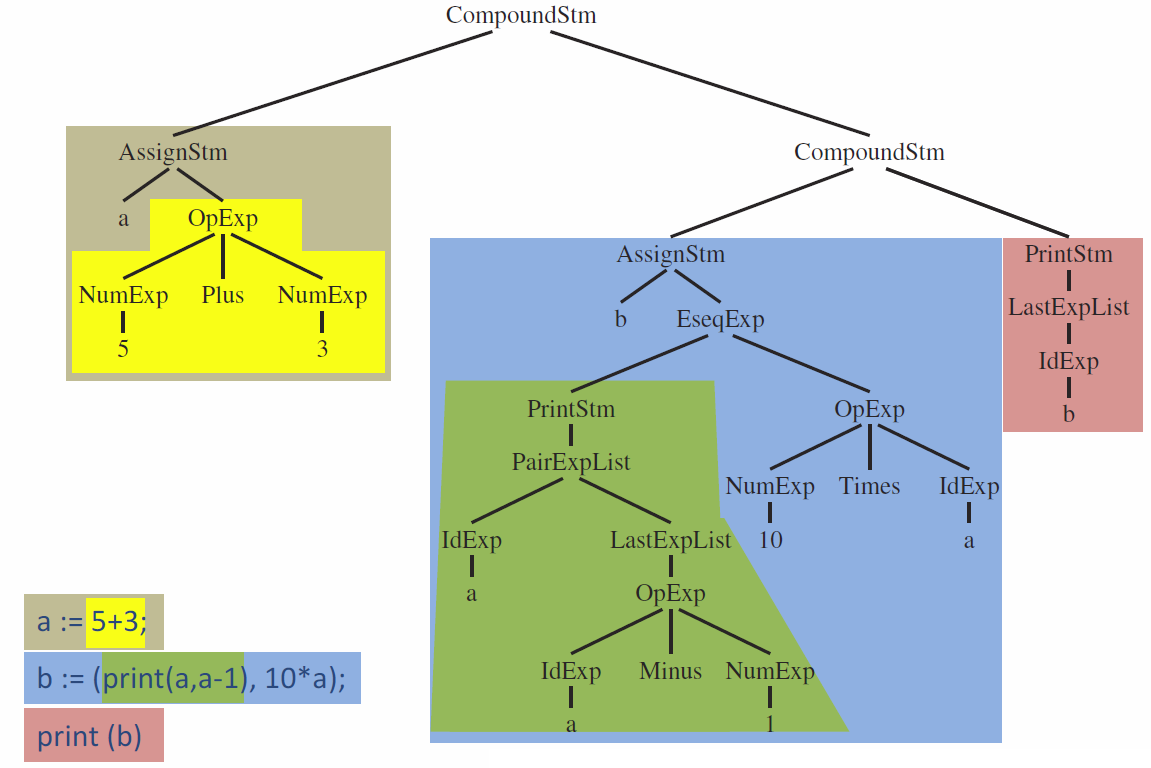
\includegraphics[width=0.8\textwidth]{abstract_syntax_tree}
	\caption{De boomvoorstelling van een eenvoudig, lusloos programma. De gekleurde deelbomen komen overeen met de gekleurde segmenten in de code zelf. Als toekenningsoperator wordt er gekozen voor $:=$ dat vanaf nu als één geheel moet beschouwd worden.}
	\label{fig:abstract_syntax_tree}
\end{figure}

\subsection{Contextvrije grammatica's}
Om een AST op te stellen moet de notie van \textbf{tokens} ingevoerd worden. Een token is eenvoudig gezien een bepaald symbool dat een betekenis heeft. De tokens van de code uit figuur \ref{fig:abstract_syntax_tree} zijn te zien in tabel \ref{table:tokens}
\begin{table}[h]
	\centering
	\begin{tabular}{l | l | l}
		symbolen(ascii) & token & waarde \\
		\hline
		a & id & string a \\
		:= & := & \\
		5 & num & integer 5 \\
		+ & + & \\
		3 & num & integer 3 \\
		; & ; & \\
		b & id & string b \\
		( & ( & \\
		print & print & \\
		- & - & \\
		* & * & \\
		  & whitespace & \\
	\end{tabular}
	\caption{De tokens die voorkomen uit het programma van figuur \ref{fig:abstract_syntax_tree}}
	\label{table:tokens}
\end{table}
Uit de theorie van de generatieve grammatica's weten we dat er zowel terminale als niet-terminale tokens bestaan:
\begin{itemize}
	\item \textbf{Terminale tokens} zijn symbolen die een blad voorstellen in de AST. Deze tokens hebben als eigenschap dat ze geen verdere tokens kunnen genereren en vormen dan ook het alfabet van het programma.
	\item \textbf{Niet-terminale tokens}, kortweg niet-terminalen genoemd, zijn de regels die de taal definiëren en zijn de niet-bladeren van de AST. Niet-terminalen hebben als eigenschap dat ze letters van het alfabet kunnen genereren.
\end{itemize}
Op figuur \ref{fig:contextvrije_grammatica} zijn een aantal terminalen en niet-terminalen te zien. De niet-terminale token \textit{CompoundStm} bestaat bijvoorbeeld uit twee \textit{Stm} tokens, gescheiden door een punt komma. Deze twee \textit{Stm} tokens kunnen in deze vereenvoudigde programmeertaal enkel een \textit{AssignStm} of \textit{PrintStm} zijn. Bij \textit{AssignStm} wordt er een terminale token verwacht in de vorm van een variabele identifier, gevolgd door de toekenningsoperator en een \textit{Exp} token. Enkel deze \textit{Exp} kan nog vier vormen aanneemen: \textit{IdExp}, \textit{NumExp}, enz...
{
\begin{figure}[h]
	\definecolor{cvred}{RGB}{215,149,146}
	\definecolor{cvblue}{RGB}{145,202,219}
	\centering
	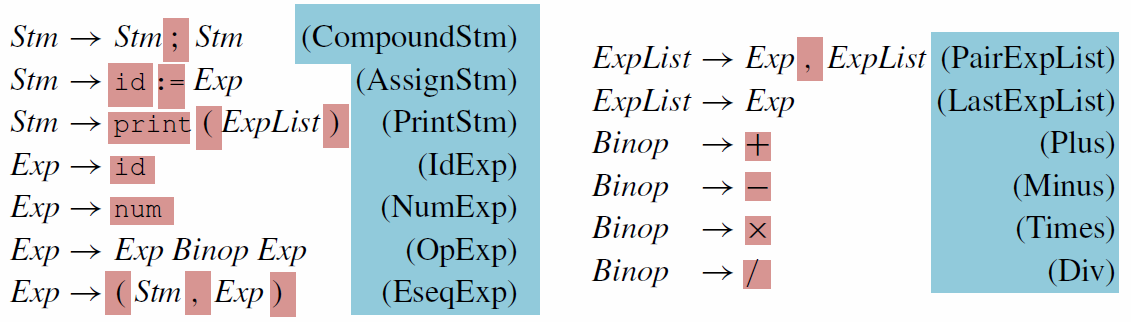
\includegraphics[width=0.8\textwidth]{contextvrije_grammatica}
	\caption{De rood omkaderde symbolen zijn {\color{cvred} terminalen} terwijl de blauw omkaderde {\color{cvblue}niet-terminalen} zijn.} 
	\label{fig:contextvrije_grammatica}
\end{figure}
}
Dit wordt uitgewerkt voor de eerste toekenningsoperatie uit figuur \ref{fig:abstract_syntax_tree} en is te zien op figuur \ref{fig:contextvrije_grammatica_voorbeeld}.
\begin{figure}[h]
	\centering
	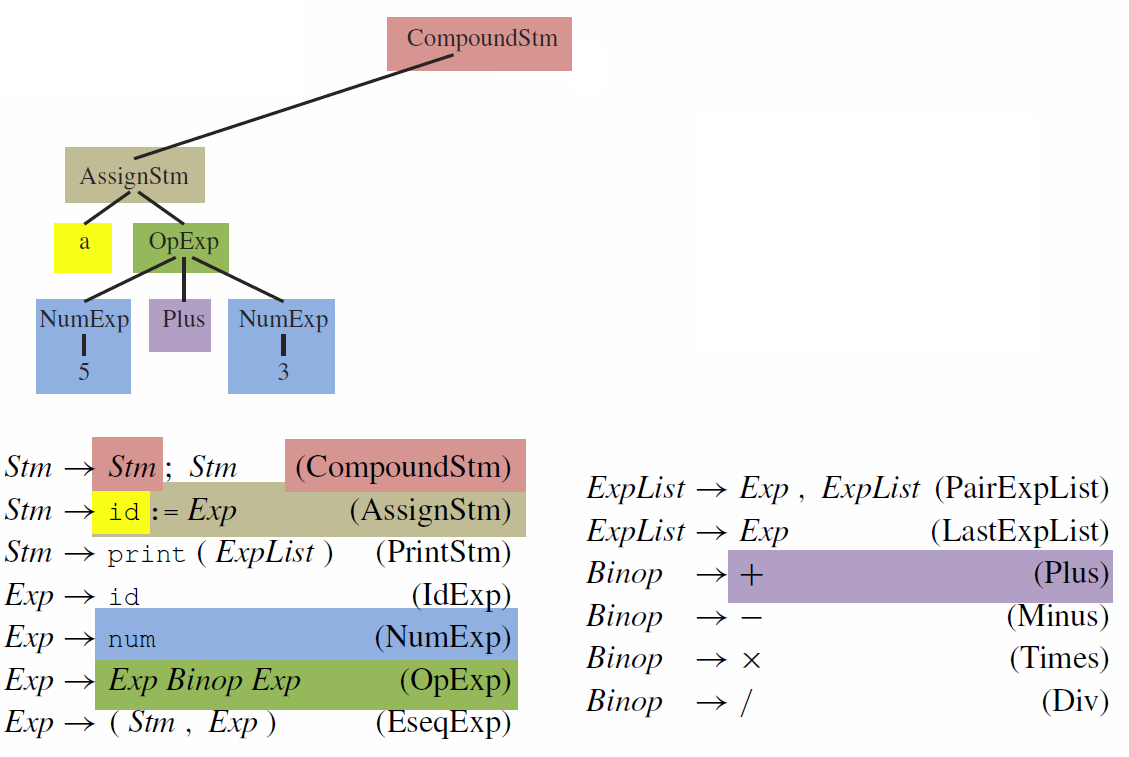
\includegraphics[width=0.8\textwidth]{contextvrije_grammatica_voorbeeld}
	\caption{Illustratie van contextvrije grammatica op de eerste toekenningsoperatie uit figuur \ref{fig:abstract_syntax_tree}.} 
	\label{fig:contextvrije_grammatica_voorbeeld}
\end{figure}

\subsection{Opbouw AST}
Een AST kan nu \textbf{bottom-up} opgemaakt worden door volgende procedure uit te voeren:
\begin{enumerate}
	\item Voor elke mogelijke knoop moet er een struct gemaakt worden zoals bijvoorbeeld:
	
	$$\texttt{A\_stm\_} \qquad \texttt{A\_exp\_} \qquad \texttt{A\_expList\_}$$
	
	\item Elke struct moet bestaan uit
	\begin{itemize}
		\item een enum voor het precieze token te bepalen,
		\item een union voor de verschillende combinaties van tokens in het rechter lid en,
		\item pointers naar kindknopen.
	\end{itemize}
	Dit wordt geïllustreerd in code \ref{lst:vb_struct_AST}.
	\begin{lstlisting}[caption={Voorbeeld van een struct voor een AST.},label={lst:vb_struct_AST}, captionpos=b]
typedef char * string;
typedef struct A_stm_ * A_stm;
typedef struct A_exp_ * A_exp;
typedef struct A_expList_ * A_expList;

struct A_stm_ {
	enum {A_compoundStm, A_assignStm, A_printStm} kind;
	union {
		struct {A_stm stm1, stm2;} compound;
		struct {string id; A_exp exp;} assign;
		struct {A_expList exps;} print;
	} u;
};
	\end{lstlisting}
	\item In de constructor worden de knopen aangemaakt, zoals te zien in code \ref{lst:vb_constructor_AST}.
	\begin{lstlisting}[caption={Voorbeeld van een constructor voor een AST.},label={lst:vb_constructor_AST}, captionpos=b]
A_stm A_CompoundStm(A_stm stm1, A_stm stm2){
	A_stm s = malloc(sizeof(*s));
	s->kind = A_compoundStm;
	s->u.compound.stm1 = stm1;
	s->u.compound.stm2 = stm2;
	return s;
}
	\end{lstlisting}
	
Op deze manier zou de boom uit figuur \ref{fig:abstract_syntax_tree} hardgecodeerd kunnen worden, wat natuurlijk geen goede manier is. Het is de taak van een \uline{lexer} en \uline{parser} om de constructie van een AST te automatiseren, die respectievelijk in hoofdstuk \ref{ch:lexicale_analyse} en \ref{ch:parsing} behandelt worden.

\subsection{Interpreter}
Uit een AST kan een eenvoudige interpreter geschreven worden. Dit stuk is informatief, en wordt niet gevraagd op het examen.
\begin{itemize}
	\item Door de boom postorder diepte-eerst te overlopen, wordt de boom in de juiste manier behandelt.
	\item Het bijhouden van de waarden van variabelen kan via een gelinkte lijst:
	\begin{lstlisting}
typedef struct table * Table_;
struct table {string id; int value; Table_ tail;};
Table_ Table(string id; int value; Table_ tail) {
	Table_ t = malloc(sizeof(*t));
	t->id = id;
	t->value = value;
	t->tail = tail;
	return t;
}
	\end{lstlisting}
	\item Stel nu dat dit de eerste drie regels van een programma zijn:
	\begin{lstlisting}
a := 2;
b := 3;
a := 3;
	\end{lstlisting}
	\item Voor de eerste toekenning bevat de gelinkte lijst slechts één knoop met als sleutel \textit{a} en waarde \textit{2}. 
	\item Bij de tweede toekenning wordt de originele gelinkte lijst meegegeven via de variabele \textit{tail}. Na deze constructor zal de gelinkte lijst twee knopen bevatten.
	\item Na deze constructor bevat de gelinkte lijst drie knopen. Merk op dat er twee knopen zijn met sleutel \textit{a}, maar dat ze elk een verschillende waarde hebben. Aangezien een nieuwe knoop vooraan wordt toegevoegd, zal de interpreter enkel de meest recentste waarde opvragen.
\end{itemize}

\end{enumerate}



	\chapter{Lexicale Analyse}
\section{Lexicale tokens}
\begin{itemize}
	\item Herkennen van een reeks opeenvolgende karakters die een geheel vormen volgens de syntax van een programmeertaal, zoals o.a:
	\begin{itemize}
		\item sleutelwoorden: int, float, for, new, ...
		\item identifiers: foo, n14, variabelenaam
		\item getallen: -37, 0x16L, 10.4, ...
		\item operatoren: +, -, *, \&, \&\&, ...
		\item andere tokens: \{ \} " ; /*  */ / ( ) [ ]
	\end{itemize}

\end{itemize}
	\chapter{Parsing}
\label{ch:parsing}

\section{Inleiding}
Het basisidee van parsing is om een string van tokens te analyseren en kijken of deze syntactisch geldig zijn.

\QA{Waarom gaan we context-vrije grammatica gebruiken in plaats van reguliere expressies om de tokens van een lexer te parsen?}{Reguliere expressies kan geen recurise uitdrukken. Ook kan de eis voor gebalanceerde haakjes niet uitgedrukt worden met reguliere expressies.
}

\section{Context-vrije grammatica}
\begin{itemize}
	\item Een \textbf{taal} is een verzameling \textbf{strings}.
	\item Een \textbf{string} is een eindige sequentie \textbf{symbolen} uit een \textbf{alfabet}.
	\item Analogie met een parser:
	\begin{itemize}
		\item De broncode levert de strings op via lexicale analyse.
		\item De lexicale tokens zijn de symbolen.
		\item Het alfabet is de verzameling tokentypes die gegenereerd worden door de lexicale analyzer.
	\end{itemize}
	\item De taal van een context-vrije
	\item Context-vrije grammatica definieert de \textbf{syntax} van de taal.
\end{itemize}

\subsection{Afleiden van een zin}
Grammatica \ref{fig:vb_grammatica_1} toont een voorbeeldsyntax voor lusloze programma's. Een voorbeeld van een zin is:

\begin{grammarfigure}
	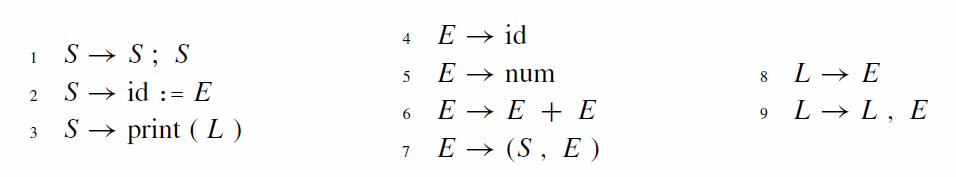
\includegraphics[width=\textwidth]{vb_grammatica_1}
	\caption{Een syntax voor een lusloos programma.}
	\label{fig:vb_grammatica_1}
\end{grammarfigure}


\begin{equation}\label{eqn:voorbeeldzin}
\texttt{id := num ; id := id + (id := num + num, id)}
\end{equation}


die bijvoorbeeld afgeleidt is door de lexer van:
$$\texttt{a := 7; b := c + (d := 5 + 6, d)}$$

Het afleiden van een zin start altijd met een \textbf{startsymbool}, die twee vormen kan aannemen:
\begin{enumerate}
	\item Het startsymbool kan enerzijds het eerste symbool zijn.
	\item Anderzijds wordt het startsymbool expliciet aangeduid zoals bijvoorbeeld $P \rightarrow S\$$, met \$ het stopsymbool.
\end{enumerate}

\begin{lstlisting}[caption={Het afleidingsproces.},label={lst:vb_afleiding},captionpos=b,escapeinside={(*}{*)}]
(*\uline{S}*)
S ; (*\uline{S}*)
(*\uline{S}*) ; id := E
id := (*\uline{E}*) ; id := E
id := num ; id := (*\uline{E}*)
id := num ; id := E + (*\uline{E}*)
id := num ; id := (*\uline{E}*) + (S, E)
id := num ; id := id + ((*\uline{S}*), E)
id := num ; id := id + (id := (*\uline{E}*), E)
id := num ; id := id + (id := E + E, (*\uline{E}*))
id := num ; id := id + (id := (*\uline{E}*) + E, id)
id := num ; id := id + (id := num + (*\uline{E}*), id)
id := num ; id := id + (id := num + num, id)
\end{lstlisting}

Code \ref{lst:vb_afleiding} toont een illustratie van hoe het afleidingsproces te werk gaat, toegepast op voorbeeldzin \ref{eqn:voorbeeldzin}. Bij elke iteratie wordt het niet-terminale token dat onderlijnt is verwerkt.

\QA{Is dit een linkse of een rechtste afleiding?}{Geen van beide, omdat er gekozen kan worden om zowel de meest linkse als de meest rechtse token te verwerken.
}

Figuur \ref{fig:vb_tree_1} toont de bijhorende parse tree. Hier zijn de bladeren ook een verzameling van terminale tokens. De taak van een parser is om de bijhorende boom op te stellen, uitgaande van enkel de bladeren.

\begin{figure}
	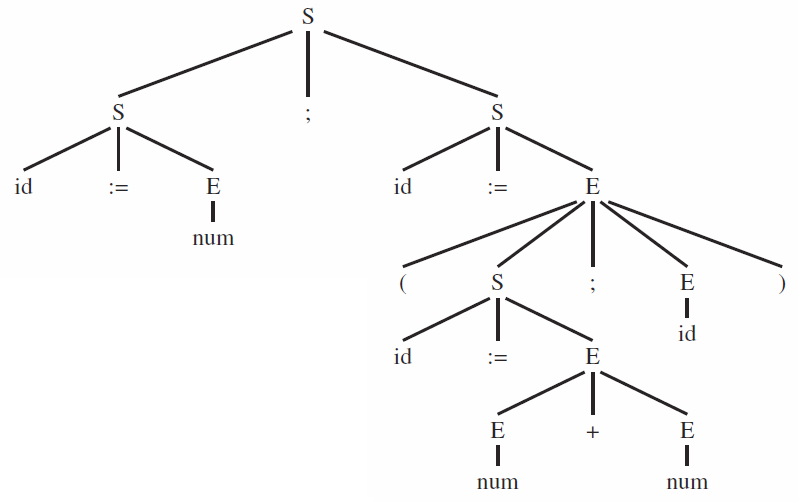
\includegraphics[width=\textwidth]{vb_tree_1}
	\caption{De bijhorende parse tree voor voorbeeldzin \ref{eqn:voorbeeldzin}.}
	\label{fig:vb_tree_1}
\end{figure}


\subsection{Ambigue grammatica}
\QA{Stel dat we Grammatica \ref{fig:vb_grammatica_1} hebben. Wat gebeurt er voor het statement \texttt{a := {\color{red}(}x + {\color{blue}(}y{\color{red})} + z{\color{blue})}}?}{Dit is een voorbeeld van een ambigue grammatica. Aan de hand van de grammatica is het onmogelijk om slechts één parse tree op te bouwen. Figuur \ref{fig:ambigious_grammar_tree} toont beide parse trees voor het statement. Bij de linkse boom worden de rode haakjes gebruikt terwijl be de rechtse boom de blauwe haakjes gebruikt worden.
}

\begin{figure}
	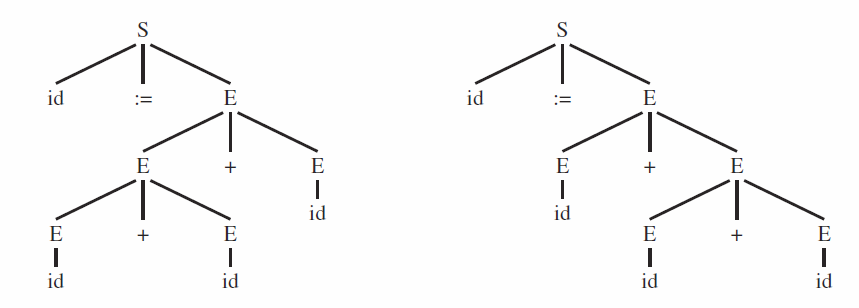
\includegraphics[width=\textwidth]{ambigious_grammar_tree}
	\caption{Voor Grammatica \ref{fig:vb_grammatica_1} kunnen er twee parse trees opgebouwd worden voor het statement \texttt{a := x + y + z}.} 
	\label{fig:ambigious_grammar_tree}
\end{figure}

Bij een plus-operatie is dit niet heel belangrijk aangezien het toch associatief is, maar bij niet-associatieve operaties is dit duidelijk niet goed.

\subsection{Grammatica disambiguëren}
Een grammatica hoeft niet perse de regels van de wiskunde te volgen. Daarom is het automatiseren ook moeilijk, omdat het afhangt van welke semantiek gewenst is. Er kan bijvoorbeeld gesteld worden dat:
\begin{itemize}
	\item * en / voorrang heeft op + en -,
	\item a + b + c = (a + b) + c, dus + is links associatief.
\end{itemize}
Om dit te realiseren worden er \textbf{termen} en \textbf{factoren} ingevoerd. Op die manier kan Grammatica \ref{grammar:3_5} omgevormd worden tot \ref{grammar:3_8}.

\begin{grammarfigure}
	\centering
	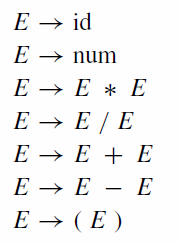
\includegraphics[width=0.25\textwidth]{grammar_3_5}
	\caption{Een ambigue grammatica. Hier wordt de regel dat * en / voorrang heeft op + en - niet gerespecteerd. }
	\label{grammar:3_5}
\end{grammarfigure}
\begin{grammarfigure}
	\centering
	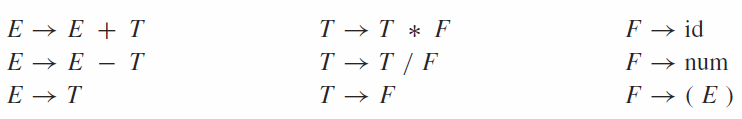
\includegraphics[width=\textwidth]{grammar_3_8}
	\caption{Grammatica \ref{grammar:3_5} kan hervormt worden, door termen $T$ en factoren $F$ in te voeren. Deze termen dwingen de volgorde van operaties en associativiteit vast.}
	\label{grammar:3_8}
\end{grammarfigure}


\section{Predictive Parsing}
Sommige grammatica's kunnen eenvoudig geparsed worden met een \textbf{recursive descent parser}. Voor elke niet-terminal is er een overeenkomstige functie. In elke functie is er een switch clause voor elke productieregel die door de niet-terminal kan gegenereerd worden. Niet-terminals worden recursief aangeroepen terwijl terminals verwerkt worden.

Code \ref{code:recursive_descent_parser} toont een voorbeld van zo een recursive descent parser toegepast op Grammatica \ref{grammar:3_11}.

\begin{grammarfigure}
	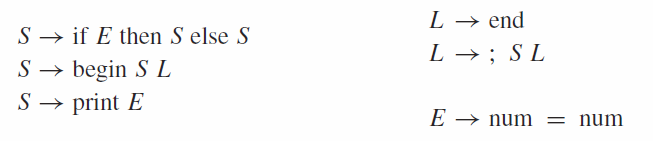
\includegraphics[width=\textwidth]{grammar_3_11}
	\caption{}
	\label{grammar:3_11}
\end{grammarfigure}

\begin{lstlisting}[caption={Een recursive descent parser gebaseerd op Grammatica \ref{grammar:3_11}},label={code:recursive_descent_parser},captionpos=b]
enum token {IF, THEN, ELSE, BEGIN, END, PRINT, SEMI, NUM, EQ};
extern enum token getToken(void);

enum token tok;
void advance() {tok = getToken();}
void eat(enum Token t) {if (tok==t) advance(); else error();}

void S(void) {switch(tok){
	case IF:    eat(IF); E(); eat(THEN); S(); eat(ELSE); S(); break;
	case BEGIN: eat(BEGIN); S(); L(); break;
	case PRINT: eat(PRINT); E(); break;
	default:    error();
}}
	
void L(void) {switch(tok){
	case END:  eat(END); break;
	case SEMI: eat(SEMI); S(); L(); break;
	default:   error();
}}

void E(void) {
	eat(NUM) ; eat(EQ) ; eat(NUM);
}
\end{lstlisting}

Een recursive descent parser werkt enkel als het eerste terminale symbool van een subexpressie genoeg informatie oplevert.

\subsection{First and follow sets}
Om de begrippen \textbf{first set} en \textbf{follow set} uit te leggen wordt Grammatica \ref{grammar:3_12} gebruikt.
\begin{grammarfigure}
	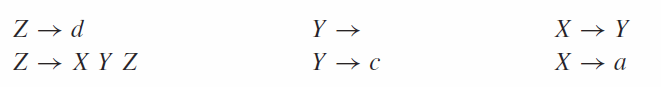
\includegraphics[width=\textwidth]{grammar_3_12}
	\caption{}
	\label{grammar:3_12}
\end{grammarfigure}
\begin{itemize}
	\item \textbf{nullable($X$)} $\rightarrow$ boolean: true als $X$ de lege string kan afleiden.
	
	We zien dat nullable($Y$) zeker waar is voor Grammatica \ref{grammar:3_12}. We kunnen echter vanuit $X$ ook naar de lege string gaan via $X \rightarrow Y \rightarrow \epsilon$, maar niet vanuit $Z$.
	
	\begin{table}[h]
		\centering
		\begin{tabular}{c | c c c}
	      & nullable & FIRST & FOLLOW \\
	      \hline
		X & yes & & \\
		Y & yes & & \\
		Z & no & & 
		\end{tabular}
	\end{table}
	
	\item \textbf{FIRST($\gamma$)}: verzameling terminals waarmee strings kunnen beginnen die van expressie $\gamma$ kunnen afgeleid worden.
	
	Uitgewerkt voor de drie startsymbolen:
	\begin{itemize}
		\item[$X:$] Vanuit $X$ zijn er twee mogelijkheden: $X \rightarrow a$ en $X \rightarrow Y$. We zien dat $a$ een terminal is dus die behoort al zeker tot de FIRST set. Vanuit $Y$ kan ook nog de lege string en $c$ bereikt worden. Hieruit volgt FIRST($X$) = $\{a\;c\}$.
		\item[$Y:$] Vanuit $Y$ kan enkel $c$ bereikt worden: FIRST($Y$) = $\{c\}$.
		\item[$Z:$] In eerste instantie kan $Z$ direct $d$ bereiken, dus die zit zeker in de FIRST set. Aangezien ook de productieregel $Z \rightarrow X\;Y\;Z$ bestaat en zowel $X$ als $Y$ nullable zijn, kan zowel de FIRST set van $X$ als van $Y$ overgenomen worden.
		
		FIRST($Z$) = $\{a\;c\;d\}$
	\end{itemize}

	\begin{table}[h]
	\centering
	\begin{tabular}{c | c c c}
			& nullable & FIRST & FOLLOW \\
			\hline
			X & yes & a c & \\
			Y & yes & c & \\
			Z & no & a c d & 
		\end{tabular}
	\end{table}
	
	\item \textbf{FOLLOW($X$)}: is de verzameling van terminals $t$ die meteen op $X$ kunnen volgen, dus waarvoor de afleiding $X_t$ bestaat. 
\end{itemize}

Algoritme \ref{algo:first_follow_nullable} is een fixpoint algoritme die de first, follow en nullable berekent.

\begin{lstlisting}[caption={Iteratieve berekening van FIRST, FOLLOW en nullable},label={algo:first_follow_nullable},captionpos=b,escapeinside={(*}{*)}]
(*\textbf{for}*) each terminal symbol Z
  FIRST[Z] (*$\leftarrow$*) {Z}
(*\textbf{repeat}*) 
  (*\textbf{for}*) each production (*$X \rightarrow Y_1Y_2...Y_k$*)
    (*\textbf{for}*) each (*$i$*) from 1 to (*$k$*), each (*$j$*) from (*$i + 1$*) to (*$k$*),
      (*\textbf{if}*) all the (*$Y_i$*) are nullable
        (*\textbf{then}*) nullable[X] (*$\leftarrow$*) true
      (*\textbf{if} $Y_1 \cdot\cdot\cdot Y_{i - 1}$*) are all nullable 
        (*\textbf{then}*) FIRST[X] (*$\leftarrow$*) FIRST[X] (*$\cup$*) FIRST[(*$Y_i$*)]
      (*\textbf{if} $Y_{i + 1} \cdot\cdot\cdot Y_{k}$*) are all nullable 
        (*\textbf{then}*) FOLLOW[(*$Y_i$*)] (*$\leftarrow$*) FOLLOW[(*$Y_i$*)] (*$\cup$*) FOLLOW[(*$X$*)]
      (*\textbf{if} $Y_{i + 1} \cdot\cdot\cdot Y_{j - 1}$*) are all nullable 
        (*\textbf{then}*) FOLLOW[(*$Y_i$*)] (*$\leftarrow$*) FOLLOW[(*$Y_i$*)] (*$\cup$*) FIRST[(*$Y_i$*)]
(*\textbf{until}*) FIRST, FOLLOW and nullable did not change in this iteration
\end{lstlisting}



\subsection{Opstellen Predictive Parsing Tabel}
Uitbreiden definitie van first naar strings:
\begin{itemize}
	\item \texttt{FIRST($W\gamma$)} = \texttt{FIRST($W$)} als niet nullable($W$)
	\item \texttt{FIRST($W\gamma$)} = \texttt{FIRST($W$)} $\cup$ \texttt{FIRST($\gamma$)} 
\end{itemize}


Er zijn drie gevallen waarbij er twee keuzes zijn. Moeten we $X \rightarrow a$ of $X \rightarrow Y$ nemen? De string $d$ levert minstens twee parse tree op. De grammatica was zelfs ambigu. Dit kan nooit geparsed worden.

\subsection{LL(1) Parsers}
\begin{itemize}
	\item Elk vak in de tabel bevat slechts 1 productieregel.
	\item Left-to-right parse: begin vooraan in broncode en verwerk van links naar rechts. 
	\item Leftmost-derivation: 
	\item 1-symbol lookahead: Er wordt slechts één symbool vooraf bekeken.
	\item LL($k$):
	\begin{itemize}
		\item $k$ symbolen vooraf bekijken. De first sets bevatten sequenties van $k$ terminals.
	\end{itemize}
	\alert Mogelijke problemen:
	\begin{itemize}
		\item Linkse recursie.
		\begin{itemize}
			\item Probleem: zekerheid van meerdere productieregels in een vak want $\texttt{FIRST(T)} \in \texttt{FIRST(E - T)}$. 
			\item Oorzaak: $E$ verschijnt links in de rechterkant van een $E$-productie.
			\item Oplossing: 
		\end{itemize} 
		\item Linkse factorisatie.
		\begin{itemize}
			\item Probleem: De parser kan geen onderscheid maken tussen twee gelijkaardige strings.
			\item Oplossing: grammatica herschrijven.
		\end{itemize}
	\end{itemize}
	\item Error recovery is mogelijk.
	\alert Beslissing nemen na $k$ symbolen blijft een zwakte.
	
\end{itemize}

\subsection{Error Recovery}
Probleem: pseudocode voor error. We willen geen compiler die geen nuttige foutboodschappen kan geven. Compiler mag ook niet stoppen bij eerste fout, omdat meerdere fouten nog verder kunnen voorkomen.
\begin{itemize}
	\item Gewoon een print statement = vrij slechte methode aangezien er geen tokens opgegeten worden. De parser doet voort alsof hij F en Tprime al geparsed heeft. De parser komt in foute toestand.
	\item Print statement combineren met de skipto functie, die tokens zal opeten totdat er een token tegenkomt die in de follow set zit. Alle karakters die niet in de follow zitten, zal nog deel uitmaken van de subexpressie. 
\end{itemize}

\section{LR(1) parser}
\begin{itemize}
	\item Left-to-right parse
	\item Rightmost-deviation
\end{itemize}
	\chapter{Abstracte syntax}
\label{ch:abstract_syntax}
Abstract syntax tree stelt eerder semantiek voor, parse trees de constructieregels. De abstract syntax tree wordt opgebouwd tijdens het parsen.
\section{Semantische acties}


Een parser voert syntactische acties uit zoals shift en reduce. Een semantische actie heeft betrekking tot de betekenis van de expressies. Het bereken van semantische waarden kan bv zijn:
\begin{itemize}
	\item het type van het linkerlid van de expressie $a = 5 + 3$ bepalen.
\end{itemize}


\subsection{Voorbeeld}
\begin{enumerate}
	\item Rekenmachine: Specifieren tokens van verschillende types (bv token type id komt overeen met strings). 
	
	Eerst $a = 5$, dan $c = a + b$, dan moet $a$ eerst opgezocht worden (lookup).
	
	Elke terminal heeft een type semantische waarde, en is dan ook returntype van de functie voor die terminal.
	
	
	\item Betere rekenmachine: niet manueel implementeren maar met tool (bv Yacc)
	
	\$\$ is de semantische waarde van het linkerlid
	
	\$1 is de semantische waarde van de eerste expressie in de tokenlijst.
	
	Figuur 4.3
	
	Semantische waarde van $exp$ is semantische waarde van $INT$
	
	Opt einde: reductie van \texttt{exp TIMES exp}
	\item Interpreter
\end{enumerate}
In feite kan compilatie uitgevoerd worden met semantische acties, maar wordt in de praktijk afgeraden:
\begin{itemize}
	\item Analyse kan enkel uitgevoerd worden in de volgorde dat de inputstream geparsed wordt. 
	\item Code genereren op basis van parse tree, maar zo een tree is niet geschikt. Er zit te veel nutteloze informatie in zoals := operator, en dient eerder om de syntax uit te drukken en niet semantiek.
\end{itemize}

\section{Abstract Parse Tree Construction}

Grammatica 4.5 is ambigue. Binaire operator specificeert geen associativiteit. Dit is geen probleem, aangezien de parser dit al beslist heeft. Dus de grammatica die de parser gebruikt mag niet ambigue zijn, wel die van de abstract syntax tree, aangezien die dient om de semantiek te definiëren.
\subsection{Posities}
Als je tree opbouwt, wordt deze geanalyseerd om bv types te checken. Bij foutboodschappen moet de compiler weten waar in de inputstroom deze fout gegenereerd wordt. Er kan een \textbf{positiestack} bijgehouden worden die de positie van elke token bevat.
	\chapter{Semantische analyse}
\label{ch:semantische_analyse}

\begin{lstlisting}
int b = 0;
extern int a;
void foobar(float b){
  if(b == 0.0){
    char * b = malloc(1);
    *b = 0;
  }
}
\end{lstlisting}

Er wordt een nullbyte weggeschreven naar $b$. Is dit een string, float, 32 bit integer, 64 bit integer? Het algemene probleem is dat er verschillende scopes zijn, en binnen elke scope kan dezelfde variabele identifier gebruikt worden. Via \textbf{symbooltabellen} wordt dit efficiënt opgelost.
\section{Symbooltabellen}
Een symbooltabel bestaat uit een \textbf{environment} $\sigma_i$ en een verzameling \textbf{bindings}.
$$\sigma_1 = \{g \rightarrow string, a \rightarrow int}$$

Elke environment $\sigma_i$ bestaat uit de samenstellingen van zijn specifieke bindings en eventueel de bindings van andere $\sigma_{j}$ voor $j \neq i$. De specifieke bindings van $\sigma_i$ hebben voorrang op de bindings van $\sigma_{j}$.

\underline{Twee implementaties:}
\begin{itemize}
	\item \textbf{Imperatieve implementatie:} Er wordt een hashtabel bijgehouden waarin kan toegevoegd en opgezocht worden. Er is geen remove operatie maar wel een pop operatie aangezien elke bucket kan gezien worden als een stapel omdat geneste expressies nooit overlappen. Elke bucket van de hashtabel is een scope.
\item \textbf{Functionele implementatie:} Kopieërt niet de hele hashtabel, maar enkel de pointers naar de relevante buckets. Kan met hashtabel, maar (zelfbalanserende) binaire zoekbomen zijn efficiënter.
\end{itemize}
\subsection{Efficiëntere symbooltabellen}
Tabel aanmaken met pointers naar identifier tijdens het parsen., in plaats van "a" op AST figuur 1.4 wordt de pointer bijgehouden in de knoop.   
(slide 15)


\section{Type Checking}
Kijken of de gebruikte veranderlijken:
\begin{itemize}
	\item gedeclareerd zijn
	\item ze van het juiste type zijn
	\item of de types van expressies correct zijn
\end{itemize}
Door de abstract syntax tree in postorder te overlopen kan dit geïmplementeerd worden. Er zullen altijd eerst declaraties bezocht worden. Er zijn verschillende visitors 
\subsection{Expressies}

\subsection{Variabelen}

\subsection{Declaraties}


	\chapter{Activation Records}
Er is een overstap nodig naar een neutrale voorstelling die onafhankelijk is van de oorspronkelijke taal. Er is wel een probleem: zelfs de omzetting van de abstract syntax tree naar deze neutrale voorstelling is afhankelijk van de architectuur waarvoor gecompileerd wordt. Bijvoorbeeld het statement \texttt{*p++} in C is anders voor 32-bit of 64-bit systemen. Het doel is om de taalspecifieke Abstract Syntax Tree om te vormen naar een taalonafhankelijke Intermediate Representation Tree.

Bij de meeste talen worden er lokale variabelen gecreëerd bij het aanroepen van een functie. Meerdere instanties van een functie kunnen bestaan en hebben elk hun eigen instanties van lokale variabelen.
\begin{lstlisting}
function f(x: int) : int =
  let var y := x + x
   in if y < 10
          then f(y)
          else y - 1
end
\end{lstlisting}
Een instantie van $x$ wordt aangemaakt elke keer dat $f$ opgeroepen wordt. Door de recursiviteit kunnen er meerdere instanties van $x$ bestaan. Een functieoproep heeft een last-in-first-out (LIFO) gedrag. Alle lokale variabelen binnen een functie worden vernietigd op het moment dat deze functie verlaten wordt. De gebruikte datastructuur is dus een \textbf{stack}.

Een hogere orde functie is een functie waarin:
\begin{itemize}
	\item een andere functie aanwezig is.
	\item een functie heeft als returnwaarde.
	\item Voorbeeld:
	\begin{lstlisting}
fun f(x) =
 let fun g(y) = x + y
  in g
 end
 
val b = f(3)
val j = f(4)
	
val z = h(5)
val w = j(7)
	\end{lstlisting}
	\good 	Zulke functies worden niet besproken in deze cursus.
\end{itemize}




\section{Stack Frames}
\begin{itemize}
	\item Een normale stack kent twee operaties: \textbf{push} en \textbf{pop}.
	\item \textbf{Problemen:}
	\begin{itemize}
		\item Lokale variabelen worden in grote hoeveelheden op de stack geplaatst. 
		\item Lokale variabelen zijn niet altijd geïnitialiseerd.
		\item Ook al zijn de variabele gepushed, is er nog steeds random access nodig.
	\end{itemize}  
	\item \textbf{Oplossing:} De stack als een array beschouwen met een speciaal register - de stack pointer. Elke lokatie na de stack pointer is rommel, alles ervoor is gealloceerd.
	\item Het gebied op de stack voor een functie $f$ die zijn lokale variabelen, parameters, returnadres en andere temporaries bevat wordt een \textbf{activation record} of \textbf{stack frame} genoemd.
\end{itemize}



Wat is het verschill tussen een caller-safed register en een callee-saved register?
\begin{lstlisting}
	ADD		R1, R2, R3 // R1 = R2 + R3
	CALL	F
	MUL		R4, R1, R7 // R4 = R1 * R7
	\end{lstlisting}
	Gaat F de waarde R1 overschrijven of niet? Als dit onbepaald is, is het geen geldige code. Een callee-saved register is de restrictie dat F deze waarde niet kan aanpassen. Een caller-safed register legt de restrictie op aan de caller van F. De assembly moet dan uitgebreidt worden:
	\begin{lstlisting}
	ADD		R1, R2, R3
	ST		R1, SP[...] // store R1 
	CALL	F
	LD      R1, SP[...] // load R1
	MUL		R4, R1, R7
	\end{lstlisting}
	Een deel van de registers worden caller-safed gemaakt, de rest is dan callee-safed. Dit wordt manueel vastgelegd. De compiler kan dan oproepen optimaliseren.






\begin{figure}
	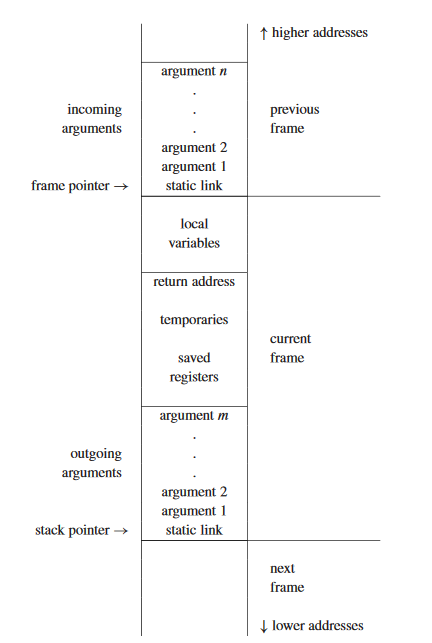
\includegraphics[width=\textwidth]{frame_layout}
	\caption{Een stack frame.}
	\label{fig:stack_frame}
\end{figure}



\subsection{Static Link}

De stack kan ook argumenten bevatten die meegegeven worden aan de functie. Een static link is vooral belangrijk bij geneste en recursieve functies. In program 6.3 (slide 6) moet de variabele \texttt{output} in elke frame beschikbaar zijn. De static link bevat een pointer naar de buitenste functie, zodat deze variabele in elke geneste functie beschikbaar is.



\subsection{Escapes}
Een variable \textit{escapet} uit een stack frame als:
\begin{itemize}
	\item hij passed-by-reference wordt.
	\item of zijn adres genomen wordt.
	\item of hij geaccessed wordt vanuit een geneste functie.
\end{itemize}

Een veranderlijke is \textit{memory-resident} (in het geheugen steken) als
\begin{itemize}
	\item hij escapet
	\item of niet in een register past
	\item of een array is
	\item of er geen vrij register is
\end{itemize}

Welke parameters moeten op de stack frame zitten en welke niet? Stel volgende functie:
\begin{lstlisting}
int f(int x, int y){
  f(x);
  g(&x);
  return x + y;
}
\end{lstlisting}
Als de functieoproepen $f$ en $g$ er niet zijn, dan moeten $x$ en $y$ niet op de stack. Bij de functie $f$ hangt het af of dat $f$ de parameter aanpast. Bij de functie $g$ moet $x$ zeker in het geheugen zitten en zal dus niet op de stack komen.
\begin{lstlisting}
int f(int x, int y){
  p = &x;
}
\end{lstlisting}


\section{Frames in de Tiger compiler}
\subsection{Frame Interface}
Er is een abstracte representatie nodig van een frame want deze hangt af van de architectuur. Deze komt in \texttt{frame.h}.

\begin{itemize}
	\item \texttt{F\_frame}: datastructuur die een frame voorstelt. 
	\item \texttt{F\_access}: datastructuur die specifieert hoe lokale variabelen moeten geaccesseerd worden (register of geheugen).
	\item \texttt{F\_accessList}: Lijst van \texttt{F\_access} structuren.
	\item \texttt{newFrame(Temp\_label name, U\_boolList formals)}: formals bevat booleans die voor elke parameter aangeeft of hij deze escapet moet worden of niet.
	\item \texttt{allocLocal(F\_frame f, bool escape)}: maakt plaats voor nieuwe veranderlijke in frame $f$, en eventueel wordt hij in het geheugen geplaatst in plaats van de stack.
\end{itemize}

Voorbeeld:
\begin{lstlisting}
F_Frame frame = F_frame(g, U_BoolList(TRUE,
                              U_BoolList(FALSE,
                                 U_BoolList(FALSE,NULL))))
\end{lstlisting}
 
\subsection{Creatie en initialisatie van frames}
\begin{figure}
	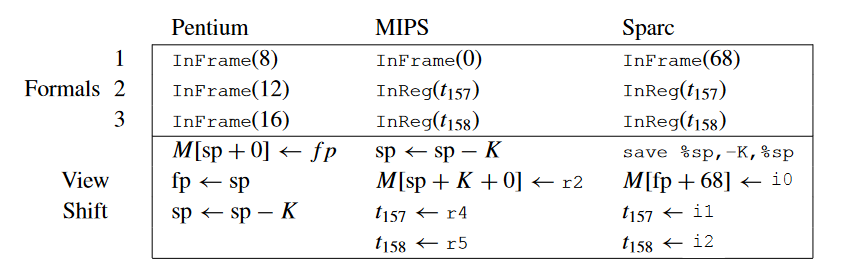
\includegraphics[width=\textwidth]{create_frames}
	\caption{Formele parameters voor $g(x_1, x_2, x_3)$ waarbij $x_1$ escapes.}
	\label{fig:create_frames}
\end{figure}

Bij Pentium moet alles op de stack. In MIPS wordt standaard de eerste 3 argumenten in registers gestoken, maar $x_1$ escapet dus wordt hij in het geheugen bewaard.
 
 \subsection{Escapes berekenen}
 Een variable \textit{escapet} uit een stack frame als:
 \begin{itemize}
 	\item hij passed-by-reference wordt.
 	\item of zijn adres genomen wordt.
 	\item of hij geaccessed wordt vanuit een geneste functie.
 \end{itemize}
 Pass-by-reference of het nemen van een referentie is direct zichtbaar in de Abstract Syntax Tree. Om na te gaan of hij geaccessed wordt vanuit een geneste functie wordt de Abstract Syntax Tree recursief overlopen met een symbooltabel (omgeving), maar hier zijn alle veranderlijken gebonden aan booleans: escapes of niet. Deze stap wordt voor semantische analyse en na parsing gedaan. Dus tussen deze twee stappen worden de escapes berekent. Het kan ook efficiënter, maar zien we niet in deze cursus.
 
\subsection{Temporaries en Labels}
\begin{itemize}
	\item Een \textbf{temporary} is een waarde die tijdelijk in een nog te bepalen register wordt bewaard.
	\item Een \textbf{label} is een nog onbekend adres waarde code of statisch gealloceerde data zal terecht komen. Bijvoorbeeld \texttt{string = \textquotedblright een string\textquotedblright} wordt statisch gealloceerd.
	\item Er is ook een aparte interface \texttt{temp.h}.
\end{itemize} 

	
\chapter{Intermediate Representations}
\begin{figure}[ht]
	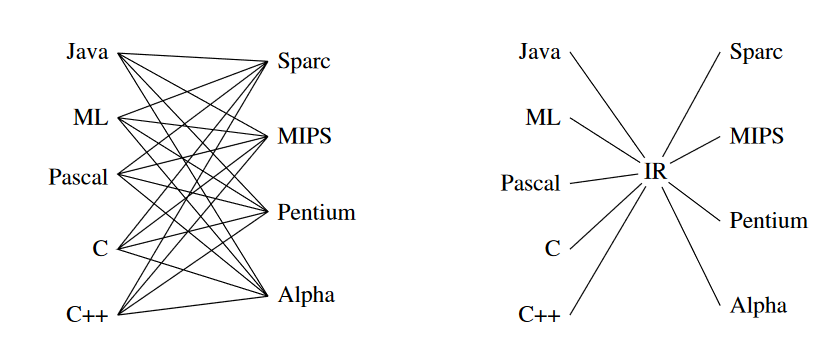
\includegraphics[width=\textwidth]{intermediate_representations}
	\caption{Compilers voor vijf talen en vier architecturen: 
		(links) geen IR, (rechts) met IR.}
	\label{fig:intermediate_representations}
\end{figure}
Een goede IR moet:
\begin{itemize}
	\item makkelijk te produceren zijn door de compiler frontend
	\item makkelijk zijn om er echte assembler van te genereren
	\item duidelijke, eenvoudige betekenis hebben
\end{itemize}

Een IR-tree is een eenvoudige abstractie van machine-instructies. Het lijkt heel goed op een Abstract Syntax Tree maar is taal-onafhankelijk en werkt met temporaries in plaats van variabelen.

Typen van expressies (\texttt{T\_exp}):
\begin{itemize}
	\item \texttt{CONST(i)}: integer constante $i$
	\item \texttt{NAME(n)}: assembly label $n$
	\item \texttt{TEMP(t)}: virtueel register $t$
	\item \texttt{BINOP(o, $e_1$, $e_2$)}: $e_1 o e_2$ met $o = +, -, *, /, ...$. Hier wordt $e_1$ altijd eerst geëvalueerd.
	\item \texttt{MEM(e)}: De inhoud van $w$ bytes op $e$ schrijven of lezen.
	\item \texttt{CALL(f, $l_1, ..., l_n$)}: roep $f$ op met argumenten $l_i$. De volgorde van de argumenten is van belang.
	\item \texttt{ESEQ(s, e)}: evalueer $s$ voor neveneffecten, dan $e$ als resultaat.
\end{itemize}

Typen van statements:
\begin{itemize}
	\item \texttt{MOVE(TEMP t, e)}: evalueer $e$ en wijs toe aan temp $t$.
	\item \texttt{MOVE(MEM($e_1$), $e_2$)}: evalueer $e_1$ tot adres $a$, evalueer $e_2$ en schijf het in de $w$ bytes vanaf $a$.
	\item \texttt{EXP(e)}: evalueer $e$ en negeer het resultaat.
	\item \texttt{JUMP(e, labs)}: evalueer $e$ tot een adres en spring er naar. 
	\item \texttt{CJUMP(e ...)}:
	\item \texttt{SEQ($s_1$, $s_2$)}: sequentie van statements 
\end{itemize}

Er is geen 1-op-1 mapping van \texttt{A\_EXP} naar \texttt{T\_EXP}.

\QA{Waarom staan er NULL pointers?}{We weten nog niet naar waar we moeten springen. Er moeten labels inkomen, maar we kennen ze nog niet. Voorlopig dienen die dus als placeholders.}

patchlist bevat de labels (in gelinkte lijst vorm) in geval van true en geval van false. De constructor bevat het hele pad in de IR tree naar het lege veld vanaf de root van het statement ($s_1$ in voorbeeld). Als de waarde 0 of 1 in \texttt{flag} moet komen kan de expressie geconverteerd worden naar een andere expressies. Program 7.3: steek 1 in temporary, als we false uitkomen wordt 0 in temporary gestoken. De doPatch functie kent een label toe aan een bepaald veld in de boom.

\subsection{Omzetting enkelvoudige veranderlijken}

$+$ symbool is dereference operator


l-values:
\begin{itemize}
	\item kan links in een toewijzing voorkomen
	\item verwijst naar een locatie
\end{itemize}

r-values:
\begin{itemize}
	\item kan enkel rechts in een toewijzing voorkomen
	\item verwijst impliciet naar een waarde
\end{itemize}

scalar:
\begin{itemize}
	\item Waarde die slechts één geheugenwoord bevat.
\end{itemize}




	\chapter{Basisblokken en traces}

Probleem met IR tree: soms is volgorde van uitvoering in de tree niet bepaald. We zouden de knopen van de IR tree kunnen herordenen.

Ander probleem: in een functiecall kan een parameter ook een functiecall zijn. De binneste functiecall moet eerst uitgevoerd worden.

Het is nog niet gemakkelijk om machinecode te genereren.


\section{Canonical trees}


\section{Linearizeren}
Door associativiteit kan de tree omgevormd worden tot een lijst van statements. Onder elke statement kunnen complexe expressies hangen in de vorm van subtrees.



\section{Basic blocks}
Algemene definitie: een sequentie van statements. Als één statement uitgevoerd wordt, moeten alle andere statements van dit block uitgevoerd worden. Een basic block start met een \texttt{LABEL} statement en eindigt met een \texttt{JUMP} of \texttt{CJUMP} statement.

\subsection{Traces aanmaken}
Een trace is een sequentie van basisblokken die mogelijk na elkaar uitgevoerd kunnen worden. De trace kan nog opgekuist worden zodat het false pad van een basisblok gevolgd wordt door zijn opvolger binnen een trace. 
\begin{itemize}
	\item Als een \texttt{CJUMP} gevolgd wordt door zijn true label kan de true en false labels omgewisseld worden. De sprongconditie moet ook geïnverteerd worden.
	\item Als een \texttt{CJUMP} niet gevolgd wordt door één van zijn labels:
	
	Vervang $$\texttt{CJUMP}(cond, a, b, t, f)$$
	
	door
	\begin{align*}
		& \texttt{CJUMP}(cond, a, b, t, f) \\
		& \texttt{LABEL}(f') \\
		& \texttt{JUMP}(\texttt{NAME} f) \\
	\end{align*}
\end{itemize}


	\chapter{Instructieselectie}

De meeste architecturen hebben complexere instructies dan degene die in de IR tree gegeven zijn. Bijna elke architectuur kan een add en een fetch uitvoeren in één enkele instructie. 
\section{Boompatronen}
Een machine-instructie is een fragment van de IR tree. Deze fragmenten worden \textbf{boompatronen} genoemd. Instructieselectie is dan het proces om de IR tree te bedekken met een minimaal aantal patronen.

\begin{figure}
	\centering
	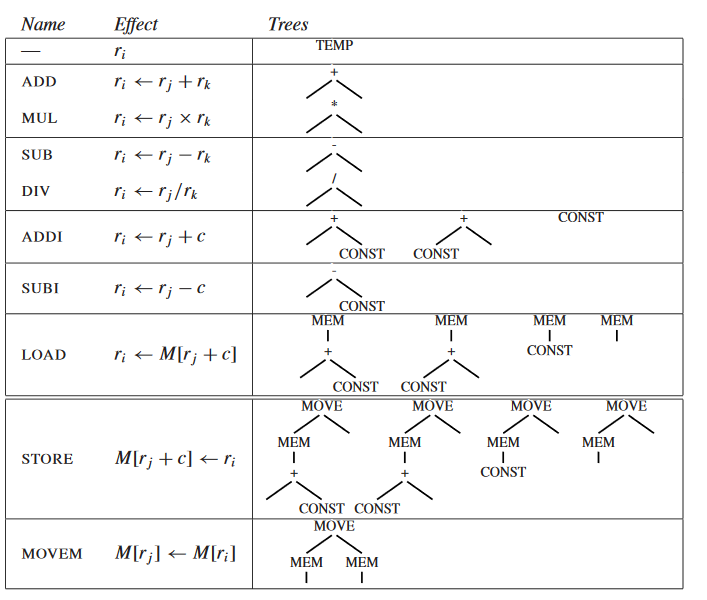
\includegraphics[width=0.7\textwidth]{jouette_instructions}
	\caption{Geheugen -en rekenoperaties. De notatie M[x] geeft het processorwoord op adress x.}
	\label{fig:jouette_instructions}
\end{figure}

Figuur \ref{fig:jouette_instructions} toont de instructieset van een \textit{uitgevonden} architectuur, \textbf{Jouette}. Elke instructie boven de dubbele lijn genereert een waarde in een register. De instructies onder de dubbele lijn bewaren niets in het register. Elke instructie heeft één of meerdere boompatronen.

Nu moet een IR tree bedekt worden met deze boompatronen. Dit heet ook \textbf{tiling} en geen enkele tile mag overlappen. Op figuur \ref{fig:tree_tiling} worden twee bomen, die identiek zijn, op een andere manier bedekt. 

\begin{figure}
	\centering
	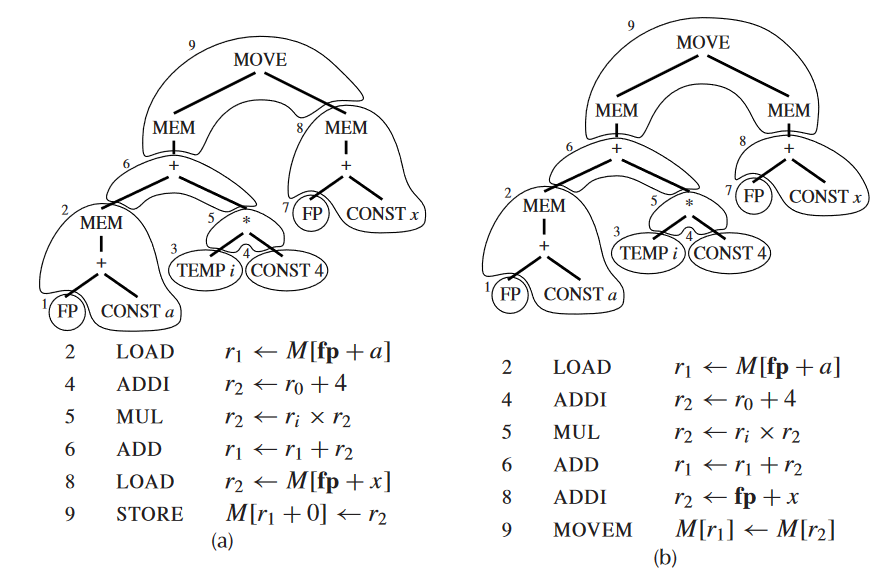
\includegraphics[width=0.7\textwidth]{tree_tiling}
	\caption{Een boom kan op meerdere manieren bedekt worden.}
	\label{fig:tree_tiling}
\end{figure}
De beste bedekking is degene die het minst 'kost'. Enerzijds kan dit het aantal instructies zijn en anderzijds de tijd die één instructie in beslag neemt. Een \textbf{optimale bedekking} wordt gedefinieerd als de bedekking waarbij:
\begin{enumerate}
	\item \textbf{optimum criterium}: de totale kost minimaal is;
	\item \textbf{optimaal criterium}: twee aaneensluitende tiles niet gecombineerd kunnen worden tot één tile met lagere kost.
\end{enumerate}
Wanneer het optimum criteria voldaan wordt, is het optimaal criteria ook automatisch voldaan. Andersom geldt het niet.

\section{Algoritmen voor instructieselectie}
\begin{table}[ht]
	\centering
	\begin{tabular}{l | l}
		RISC & CISC \\
		32 registers & weining registers \\
		Register-register architectuur & Memory-memory architectuur \\
		3-adresinstructies: R1 $\rightarrow$ R2 op R3 & 2-adresinstructies: R1 $\rightarrow$ R1 op R2 \\
		1 adresseermode & veel adresseermodes \\
		Vaste instructielengte & variabele instructielengte \\
	\end{tabular}
\end{table}

\subsection{Maximal Munch}
Het algoritme voor optimale bedekking heet \textbf{Maximal Munch}:
\begin{enumerate}
	\item Begin bij de wortel van de boom en zoek de grootste tile dat past. De grootste tile is degene met het meest knopen. Als er meerdere tiles zijn met hetzelfde aantal knopen, wordt er random gekozen.
	\item Bedek de wortel, en eventueel andere knopen, met deze tile.
	\item Er onstaan nu deelbomen, waarop hetzelfde principe kan toegepast worden.
\end{enumerate}

\subsection{Dynamisch programmeren}
De optimale bedekking is NP-compleet. Het Maximal Munch algoritme zal altijd aan het optimaal criterium voldoen, maar niet aan het optimum criterium. Om het optimum criterium toch te laten voldoen, wordt dynamisch programmeren gebruikt. In deze versie krijgt elke knoop een kost die gelijk is aan de som van de laagste instructiekosten van de deelboom waarvan de knoop wortel is, bedekt kan worden. Het algoritme loopt nu als volgt:
\begin{enumerate}
	\item Bereken de kost van elke knoop bottom-up. De kost van een knoop $n$ wordt bepaald door eerst de kost van zijn kinderen, kleinkinderen, enz... te bepalen. 
	\item Elke tile wordt nu gematched tegen node $n$. Voor elke tile $t$ met kost $c$ that op $n$ gelegd kan worden zullen er nul of meer deelbomen $d_i$ zijn die overeenkomen met de bladeren van deze tiles. Een blad van een tile zijn knopen waaraan een deelboom kan aangehangen worden. De kost $c_i$ van elke deelboom is reeds gekend, dus de kost van tile $t$ is $c + \sum c_i$.
	\item Voor elke tile $t_j$ dat $n$ kan bedekken, diegene met de minimale kost wordt gekozen.
\end{enumerate}

	\chapter{Liveness analyse}
\label{ch:liveness_analyse}

Dit is een vorm van een \textit{dataflow} analyse. Hoofdstuk \ref{ch:data_flow_analysis} bespreekt andere \textit{dataflow} analyses.

\section{Control Flow Graphs}
Een \textbf{Control Flow Graph (CFG)} is een niet-lineaire voorstelling van de assemblycode die uitgevoerd wordt. Elke instructie wordt een knoop in de CFG.

\begin{figure}[ht]
	
	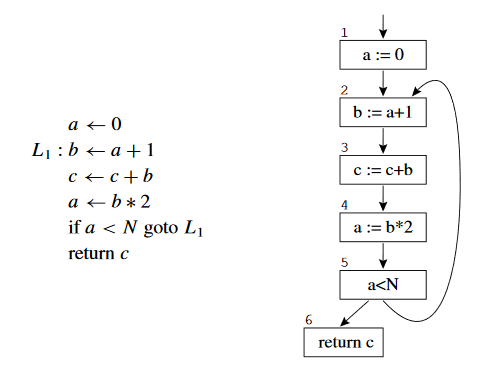
\includegraphics[width=\textwidth]{cfg_example}
	\caption{De CFG van een programma.}
	\label{fig:cfg_example}
\end{figure}


\QA{Hoeveel registers zijn er nodig om de temporaries $a$, $b$ en $c$ bij te houden voor het programma in figuur \ref{fig:cfg_example}? De variabele $c$ is een parameter die meegegeven wordt aan de functie.}{
Eerst afvragen waar in het programma de waarde van deze variabelen een rol kunnen spelen. 
}

Voor de variabele $a$ kan nagegaan worden waar de waarde nodig is. Er is sprake van vijf verschillende sets:
\begin{itemize}
	\item \textbf{in set}:  De in set geeft voor instructie $x$ de variabelen die nodig zijn van instructie $x - 1$. Zo is in[2] = \{a, c\}.
	\item \textbf{out set}: De out set geeft voor instructie $x$ de variabelen die nodig zijn voor instructie $x + 1$. Zo is out[1] = \{a, c\}.
	\item \textbf{def set}: De def set geeft voor instructie $x$ de variabelen die gedeclareerd worden door instructie $x$. Zo is def[1] = \{a\}.
	\item \textbf{use set}: De use set geeft voor instructie$x$ de variabelen die gebruikt worden door instructie $x$. Zo is use[2] = \{a, b\}.
	\item \textbf{succ set}: De succesor set geeft voor instructie $x$ de instructies die op instructie $x$ kunnen volgen. Zo is succ[5] = \{2, 6\}.
\end{itemize}

Figuur \ref{fig:use_defs} toont de verschillende locaties waar de waarde van $a$ vereist is.

\begin{figure}[ht]
	\centering
	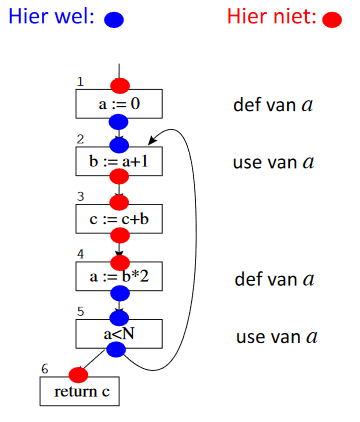
\includegraphics[width=0.5\textwidth]{use_defs}
	\caption{De plaatsen waar de waarde van $a$ een rol speelt.}
	\label{fig:use_defs}
\end{figure}

De \textbf{in} en \textbf{out} sets kunnen bekomen worden met volgende vergelijking:
\begin{align*}
	in[n] & = use[n] \cup (out[n] - def[n]) \\
	out[n] & = \bigcup_{s \in succ[n]} in[s]
\end{align*}

Via de \textbf{in} en \textbf{out} set kan de \textbf{liveness range} van elke variabele bepaald worden:
\begin{align*}
in[1] & = \{c\} \\
out[1] & = \{a, c\}\\
in[2] & = \{a, c\}\\
out[2] & = \{b, c\}\\
in[3] & = \{b, c\}\\
out[3] & = \{b, c\}\\
in[4] & = \{b, c\}\\
out[4] & = \{a, c\}\\
in[5] & = \{a, c\}\\
out[5] & = \{a, c\}\\
in[6] & = \{c\}\\
out[6] & = \{ \}
\end{align*}

Dit kan gevisualiseerd worden in de CFG (figuur \ref{fig:liveness_visual}).
\begin{figure}[ht]
	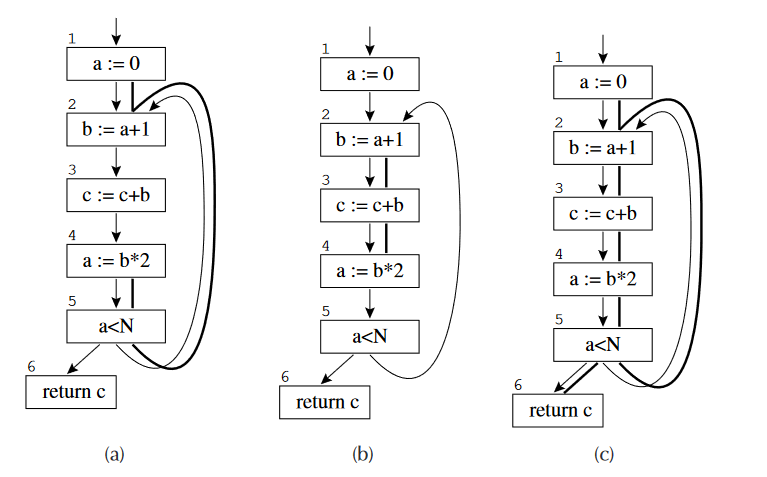
\includegraphics[width=\textwidth]{liveness_visual}
	\caption{Liveness van de variabelen $a, b$ en $c$.}
	\label{fig:liveness_visual}
\end{figure}

De vergelijking kan opgelost worden via een algoritme.
\begin{itemize}
	\item Iteratief algoritme
	\item Itereer over alle blokken in de graaf in omgekeerde volgorde (van onder naar boven).
	\begin{itemize}
		\item Maak kopie van de in en out sets
		\item Bereken de nieuwe in set
		\item Bereken de nieuwe out set
	\end{itemize}
	\item Blijf dit doen zolang er een set gewijzigd wordt.
\end{itemize}

Complexiteit:
\begin{itemize}
	\item Stel programmagrootte: $N$ statements.
	\item Elk statement kan maar 1 veranderlijke updaten, dus maximum $N$ veranderlijken.
	\item De set operatie is $O(N)$.
	\item De for loop is dan $O(N^2)$.
	\item In elke iteratie minsten 1 element toevoegen door een monotone update, dus max $2N^2$ iteraties van de repeat loop.
	\item Complexiteit: $O(N^4)$.
	\item In realiteit is het bijna lineair.
\end{itemize}

Voorstellingen van sets:
\begin{itemize}
	\item Eenvoudigste voorstelling van een set: bitvectoren. Bijvoorbeeld 64 bits, als bit 3 op 1 staat, zit 3de temporary in de s
	\item Als er te veel temporaries zijn kan gelinkte lijst gebruikt worden.
\end{itemize}


\section{Least Fixed Point \& Conservativiteit}
Er zijn meerdere oplossingen van de liveness vergelijkingen. De meest conservatieve oplossing zet alle variabelen op live bij elke instructie. 

\QA{Kan $Y$ een probleem geven? Kan $Z$ een probleem geven? (Slide 13)}{De $Y$ analyse zal nog steeds een correct programma opleveren, maar het is niet optimaal. De $Z$ analyse zal registers overschrijven.}

Een analyse is conservatief als het gedrag van het programma niet gewijzigd wordt.


\section{Statische approximatie}
Er is een verschil tussen \textbf{dynamische liveness} en \textbf{statische liveness}:
\begin{itemize}
	\item Dynamische liveness: Een variabele $a$ is dynamisch live in node $n$ als er een instructie van het programma bestaat van $n$ naar een \textit{use} van $a$ dat niet door een \textit{def} van $a$ gaat.
	\item Statische liveness: Een variabele $a$ is statisch live in node $n$ als er een pad bestaat van controle-flow verbindingen van $n$ naar een \textit{use} van $a$ dat niet door een \textit{def} van $a$ gaat.
\end{itemize}


\section{Interference Graph}
We zijn enkel geïnteresseerd welke sets meerdere veranderlijken bevat. De interference graph verbindt knopen die samen kunnen voorkomen.
\begin{figure}[ht]
	\centering
	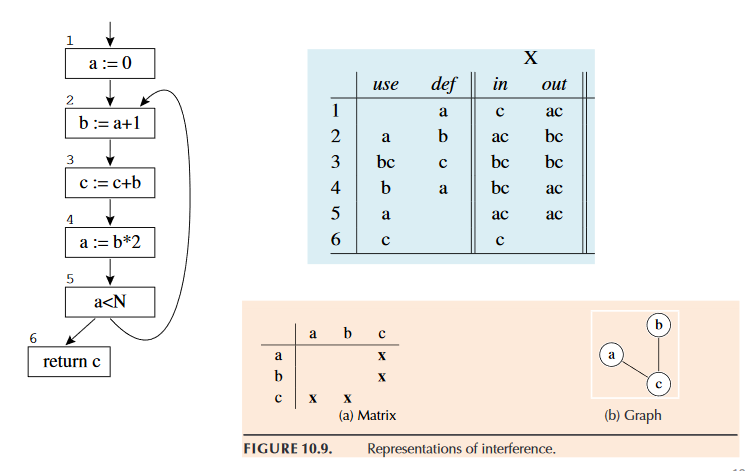
\includegraphics[width=\textwidth]{interference_graph}
\end{figure}
	\chapter{Registerallocatie}
Graph coloring om registers te alloceren in een interference graph.


Met sommige knopen geen rekening houden (bv h, want er zullen toch twee kleuren overblijven want heeft maar 2 buren).

\begin{enumerate}
	\item Vereenvoudig de graaf door continue knopen met een graad $< k$ weg te laten. Steek ze op een stack.
	\item Pop and color: selecteer een kleur en voeg knoop terug toe met die kleur aan de graaf.
\end{enumerate} 

\section{Register Coalescing}
Knopen die kopieën bevatten proberen samen te voegen als die het kleuren hoogstwaarschijnlijk niet bemoeilijken.

Twee heuristieken die het kleuren zeker niet moeilijker maken:
\begin{itemize}
	\item heuristiek van Briggs: als samengevoegde knoop minder dan $K$ buren van significante graad heeft
	\item heuristiek van George: Elke buur $t$ van $a$ is ofwel een buur van $b$ ofwel niet van significante graad.
\end{itemize}

Figuur \ref{fig:graph_coalescing} illustreert het algoritme en bestaat uit een aantal operaties.

\begin{figure}
	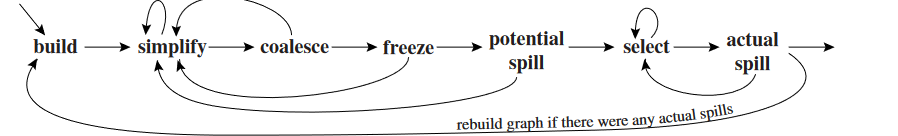
\includegraphics[width=\textwidth]{graph_coalescing}
	\caption{Graafkleuring met \textit{coalescing}.}
	\label{fig:graph_coalescing}
\end{figure}

\begin{itemize}
	\item \textbf{Build:} Construeer de interferentiegraaf en markeer elke knoop als \textit{move-related} of \textit{non-move-related}. Een \textit{move-related} knoop is een knoop dat ofwel het doel of de bron is van een \textit{move} instructie.
	\item \textbf{Simplify:} Verwijder iteratief één \textit{non-move-related} knoop die  graad minder dan $K$ heeft.
	\item \textbf{Coalesce:} Pas \textit{conservative coalescing} toe op de gereduceerde graaf met behulp van Briggs of George. \textbf{Simplify} en \textbf{Coalesce} wordt uitgevoerd tot dat er 
	\item \textbf{Freeze:}
	\item \textbf{Potential Spill:}
	\item \textbf{Select:}
	\item \textbf{Actual spill:}
\end{itemize}
	\chapter{Data Flow Analysis}
\label{ch:data_flow_analysis}
Compilers maken programma's kleiner, sneller. Zelfs perfecte $C++$ code kan nog steeds verbeterd worden. Een ontwerper van een programmeertaal gaat ervan uit dat een compiler veel \textit{under the hood} functies heeft.


\section{Analyse en transformaties}
\begin{itemize}
	\item Verzamel informatie
	\item Controleer de eigenschappen (precondities)
	\item Voer de transformatie uit
\end{itemize}

Interproceduraal = van meerdere procedures informatie verzamelen zodat een functie eigenschappen kan bevatten van andere functies.

Lokaal = slechts één blok wordt bekeken in een functie

Globaal = alle blokken in een functie wordt bekeken


\begin{lstlisting}
a = 1
b = a
a = 2
c = a
\end{lstlisting}
Welke waarde zit in $c$? 

Flow insensitief = slechts één eigenschap bijhouden per variabele.
\begin{lstlisting}
a = ?
b = ?
\end{lstlisting}

Flow sensitief = per blok in het programma eigenschappen bijhouden
\begin{lstlisting}
a1 = 1
b = a1
a2 = 2
c = a2
\end{lstlisting}

als een blok van meerdere paden kan bereikt worden, kan een variabele meerdere waarden aannemen.
Pad insensitief =  geen rekening houden met het pad, zodat we niet weten welke waarde een variabele heeft



Pad sensitief = Wel rekening houden met de verschillende paden


Voorbeeld slide 4
\begin{itemize}
	\item Javacode
	\item In veld $f$ van type $A$ kan ofwel object van type $B$ of $C$ zitten.	
	\item De \texttt{toString()} methode kan ofwel die van $B$ of van $C$ oproepen. Maar het is duidelijk dat het van type $B$ is, dus er is iets fout gelopen in de analyse.
	\item Voeg virtuele klassen $A1$ en $A2$ toe die beiden een attribuut $f$ hebben die respectievelijk een object van type $B$ en $C$ kunnen hebben.
	\item Het object $o$ zal nu zeker weten dat de toString() van object $B$ opgeroepen moet worden.
\end{itemize}


Niet altijd nuttig om zo sensitief mogelijk te gaan = te veel geheugen nodig.


\section{Verschillende dataflow analyses}
\subsection{Reaching definitions}
\begin{itemize}
	\item Nagaan of een toekenning aan een temporary $t$ de waarde van $t$ op een andere punt in het programma wijzigt.
	\item Een \textbf{niet-ambigue} definitie van $t$ is een statement van de vorm:
	\begin{itemize}
		\item $t \leftarrow a + b$, of 
		\item $t \leftarrow M[a]$;
		\item Een niet-ambigue definitie $d$ bereikt een statement $u$ zals er een pad van $d$ naar $u$ bestaat waarop geen niet-ambigue definitie van $t$ voorkomt.

	\end{itemize}
	\item Een \textbf{ambigue} definitie is een statement dat al dan niet een waarde aan $t$ toekent. \uline{Er wordt verondersteld dat elke definitie niet-ambigue is.}
	\item Om de \textit{reaching definitions} te bepalen wordt er gebruik gemaakt van een \textbf{gen[n]} set en \textbf{kill[n]} set, die beiden een lijst van statements bevat voor elk statement.
	\begin{itemize}
		\item Een statement $d_1 : t \leftarrow x \oplus y$ genereert de definitie $d_1$, want elke andere definitie van $d_1$ die dit statement bereikt wordt toch ongedaan gemaakt.
		\item Een statement $d_1 : t \leftarrow x \oplus y$ \textit{kills} elke andere definitie van $t$ want elke andere definitie van $t$ is ongeldig na dit statement.
	\end{itemize}
	\item Via \textit{gen} en \textit{kill} kunnen de \textbf{in[n]} set en \textbf{out[n]} set bepaald worden; de set van definities die respectievelijk het begin en einde van een statement $n$ bereiken. Deze sets kunnen bepaald worden door de \textit{dataflow} vergelijkingen.
	\begin{align*}
		in[n] & = \bigcup_{p \in pred[n]} out[p] \\
		out[n] & = gen[n] \cup (in[n] - kill[n])
	\end{align*}
	\item Deze vergelijkingen moeten \textbf{voorwaards} opgelost worden (in volgorde van programma, in tegenstelling tot liveness analyse, die in omgekeerde volgorde werkt).
	\item Met behulp van reaching definitions kan bijvoorbeeld nagegaan worden of een variabele uninitialized is, of variabelen vervangen door constanten (\textit{constant propagation}).

\end{itemize}

\subsection{Available expressions}
\begin{itemize}
	\item Nagaan of een bepaalde expressie meerdere malen berekend wordt met dezelfde parameters.
	\item Een expressie $x \oplus y$ is \textit{available} (bereikbaar) in statement $n$ als er op elk pad van het begin van het programma tot aan $n$ als:
	\begin{itemize}
		\item de expressie minstens éénmaal berekend wordt, en
		\item als er geen definities zijn van $x$ of $y$ vanaf de laatste keer dat de expressie berekend wordt.
	\end{itemize} 
	\item Ook hier zijn er \textbf{gen[n]} en \textbf{kill[n]} sets, maar in plaats van definities bevat het nu expressies.
	\item Opnieuw worden de \textbf{in[n]} en \textbf{out[n]} sets bepaald; de set van expressies die respectievelijk het begin en einde van een statement $n$ bereiken. Het enige verschil met \textit{reaching definitions} is dat nu de \textbf{intersectie} genomen wordt in plaats van de \textbf{unie}. Dit is nodig omdat de expressie op elk pad berekend moet worden.
	\begin{align*}
		in[n] & = \bigcap_{p \in pred[n]} out[p] \\
		out[n] & = gen[n] \cup (in[n] - kill[n])
	\end{align*}
	\item Deze vergelijkingen moeten ook \textbf{voorwaards} opgelost worden.
	\alert Omdat we met de intersectie werken (zal sets kleiner maken), moet de \textbf{out} set geïnitialiseerd worden als de volledige set van expressies.
\end{itemize}
\subsection{Reaching expressions}
Hetzelfde als reaching definitions, maar met expressies.
\subsection{Liveness analyse}
\begin{itemize}
	\item Zelfde als hoofdstuk \ref{ch:liveness_analyse}.
	\item Maar $use[n] = gen[n]$ en $def[n] = kill[n]$.
	\item Logisch aangezien elke \textit{use} liveness genereert, en elke \textit{def} liveness killt.
\end{itemize}


\section{Optimalisaties}
\begin{itemize}
	\item Common-subexpression elimination
	\begin{itemize}
		\item In plaats van nieuwe berekeningen uit te voeren, gebruik het resultaat van vorige berekeningen.
		\item \textbf{Formeel}: voor een statement $s : t \leftarrow x \oplus y$ waarbij de expressie $x \oplus y$ \textit{available} is, kan de bewerking voor $s$ geëlimineerd worden.
		\item \textbf{Algoritme}:
		\begin{enumerate}
			\item Bereken de \textit{reaching expressions} voor $s$.
			\item Voor elke statement $n$ in de reaching expression set van $s$:
			\begin{itemize}
				\item Kies een nieuwe temporary $w$
				\item Herschrijf:
				\begin{align*}
					n  & : w \leftarrow x \oplus y \\
					n' & : v \leftarrow w
				\end{align*}
			\end{itemize}
			Statement $s$ kan nu herschreven worden:
			$$s : t \leftarrow w$$
		\end{enumerate}
		\item Met \textit{constant propagation} worden sommige assignments vereenvoudigd.
	\end{itemize}
	\item Constant propagation
	\begin{itemize}
		\item Stel een statement $d : t \leftarrow c$ waarbij $c$ een constante is.
		\item Stel een andere statement $n : \leftarrow t \oplus x$
		\item Als statement $d$ statement $n$ bereikt, en er geen definities van $t$ het statement $n$ bereiken, dan kan $t$ vervangen worden door de constante waarde.

		
	\end{itemize}
	\item Copy propagation
	\begin{itemize}
		\item Zelfde princiepe als constant propagation, maar met een variabele $z$.
		\alert Waarom niet gewoon coalescing tijdens register allocation?
		\begin{itemize}
			\item Omdat sommige optimalisatiemogelijkheden  verdwijnen
		\end{itemize}
	\end{itemize}
	\item Dead code elimination
	\begin{itemize}
		\item Ergens een definitie die nooit gebruikt wordt
		\item Statement schrappen.
	\end{itemize}
\end{itemize}

Deze optimalisaties worden iteratief uitgevoerd: het toepassen van een optimalisatie laat nieuwe optimalisaties toe.

\section{Snellere analyses}

\begin{enumerate}
	\item Bitvectors
	\item Slechts voor elk basic blok toepassen (statements samenvoegen die slechts 1 successor en 1 predecessor hebben). 
	\begin{itemize}
		\item Voorbeeld \textit{reaching definitions}
		\begin{align*}
			out[n] & = gen[n] \cup (in[n] - kill[n]) \\
			out[n] & = gen[n] \cup ((gen[p] \cup (in[p] - kill[p])) - kill[n]) \\
			out[n] & = gen[n] \cup (gen[p] - kill[n]) \cup (in[p] - (kill[p] \cup kill[n]))
		\end{align*}
		Voor een knoop $pn$ dat knoop $p$ en $n$ combineert, dan komt dit neer op:
		\begin{align*}
			gen[pn] &= gen[n] \cup (gen[p] - kill[n]) \\
			kill[pn] &= kill[p] \cup kill[n]
		\end{align*}
	\end{itemize}

	\item Volgorde van toepassen aanpassen (zie algoritme onderaan slide 15)
	\item Er wordt enkel de out set bijhouden, de inset wordt telkens opnieuw berekend omdat die vaak kleiner zijn, zodat er minder geheugen nodig is om al de sets bij te houden.
	\item chains 
	\begin{itemize}
		\item use def  = bijhouden van alle reaching definitions van een temporary
		\item def use = omgekeerd
	\end{itemize}
	\item Work-list algoritme houdt bij waar er nog berekeningen nodig kunnen zijn. (algoritme 17.6)
\end{enumerate}

\section{Incrementele analyses}
Elke transformatie heeft invloed op resultaten van de analyse. Moeten we dan de hele analyse opniew doen? Als $z$ dood is, moet van onder naar boven elke keer het statement verwijderd worden bij elke iteratie.

\subsection{Value Numbering}
Elke expressie een nummer geven en hergebruiken van die expressies.

\subsection{Incremente livenessanalyse}
Veel te moeilijk om te implementeren, wordt bijna nooit gebruikt.

\section{Alias Analysis}
Niet in detail te kennen

Kunnen $p$ en $q$ naar hetzelfde object wijzen (may-alias informatie)?
Wijst $p$ en $q$ naar hetzelfde object (must-alias informatie)? 

Een zeer moeilijke analyse en hebben maar een beperkte precisie (in bv $C$ en $C++$)

Herordenen van geheugenoperaties: waarom is dit van zo een groot belang? voor parallelisatie.
	\chapter{Loop Optimizations}

Formele definitie van een lus: verzameling knoepn $S$ met daarin een header $h$, vanuit elke knoop in de lus kan je naar $h$, van $h$ kan je naar elke knoop in $S$, externe pijlen komen enkel toe in $h$.

De knopen in een lus vormen een \textit{strongly connected component}: vanuit één knoop in de lus kan elke andere knoop in de lus bereikt worden. De back edge is de verbinding die de een knoop naar de header verbindt

Reduceerbaarheid = niet te kennen. Enkel weten dat lussen volledig overlappen of helemaal niet. Ze kunnen niet deels overlappen.

\section{Dominators}
\begin{itemize}
	\item Veronderstel 1 startknoop $s_0$ van de $CFG$.
	\item Knoop $d$ domineert knoop $n$ als elk pad van $s_0$ naar $n$ door $d$ gaat.
	\item Eenvoudig berekenen met data flow analyse. Hoe initialiseren? maximale sets. 
	\item In plaats van data  flow analyse kan ook de dominator tree opgesteld worden. De dominator set van een knoop is dan de opeenvolging van ouderknopen.
\end{itemize}

Eigenschappen van een dominator:
\begin{itemize}
	\item Transitief: $a$ dom $b$ en $b$ dom $c$ $\rightarrow a$ dom $c$.
	\item Als $e$ dom $n$ en $d$ dom $n$, dan $e$ dom $d$ of $d$ dom $e$.
	\item Elke knoop $n$ heeft een unieke immediate dominator \texttt{idom($n$)}
\end{itemize}

\subsection{Header loops}
\begin{itemize}
	\item Een header $h$ kan header zijn van meerdere lussen.
	\item Loops kunnen genest zijn.
	\item Een loop-nest tree geeft aan welke knopen op welk loopniveau ze zitten.

\end{itemize}

\subsection{Loop preheader}
\begin{itemize}
	\item Algemene code die voor een lus moet uitgevoerd worden.
	\item Handig als er meerdere paden naar de header van de lus zijn.
\end{itemize}



\section{Loop Invariant Computations}
\begin{itemize}
	\item Berekeningen die altijd dezelfde waarde hebben kunnen buiten de lus geplaatst worden. (! niet altijd, soms is herberekenen beter dan de registers te gebruiken)
	\item Een definitie $d : t \leftarrow a_1 op a_2$ is loop-invariant als voor elke $a_i$:
	\begin{itemize}
		\item $a_i$ een constante is;
		\item alle definities van $a_i$ die $d$ bereiken bevinden zich buiten de lus;
		\item of de enige definitie van $a_i$, die $d$ bereikt, loop-invariant is.
	\end{itemize}
\end{itemize}

Voorbeelden: mogen we $t \leftarrow a + b$ voor de loop zetten?

Oppassen met side-effects: exceptions, pointer dereferencing

\subsection{Conversie lussen voor LCIM}



\section{Inductieveranderlijken}




\section{Loop unrolling}
	\chapter{Static Single-Assignment}
Dient om eenvoudiger Data-Flow analyse te doen. Maar er moet wel eerst Control-flow analyse gedaan worden.


Use-def chain = per gebruik van een veranderlijke (statement 2, voor veranderlijke a) bijhouden waar deze gedefinieerd wordt (in statement 1). Nog altijd niet optimaal: vezameling van meerdere elementen zijn nog  steeds mogelijk. Idealiter wordt er maar één (of zelfs geen) statement bijgehouden = Single Assignment Form.


Static Single Assignment = zorgen dat een veranderlijke op slechts één plaats geïnitialiseerd wordt. Voordelen:
\begin{itemize}
	\item De dataverloopanalyse wordt gemakkelijker.
	\item De analyses verlopen nu lineair.
	\item Ontkoppeling veranderlijken met dezelfde naam. De programmeur heeft zelf drie keer de variabele $a$ gebruikt, maar kan even goed andere variabelenamen zijn.
\end{itemize}

De $\phi$-functie geeft $a_2$ terug als het programma van blok $3$ komt en $a_1$ als het programma van blok $2$ komt. Elke veranderlijke wordt nu slechts éénmaal gedefinieerd.

Hoe $\phi$-functie wegwerken? Voeg move operaties toe na blok 3 en 2 die respectievelijk $a_2$ en $a_1$ in $a_3$ steken.

Wanneer $\phi$-functie toevoegen?
\begin{itemize}
	\item $a_i$ = $\phi(a_1, ..., a_n)$ is nodig in blok $z$ als
	\begin{itemize}
		\item $a$ gedefinieerd in blok $x$
		\item $a$ gedefinieerd in blok $y \neq x$
		\item Pad van pijlen van $x$ naar $z$ ($P_{xz}$) is niet leeg
		\item Pad van pijlen van $y$ naar $z$ ($P_{yz}$) is niet leeg	
		\item $P_{xz}$ en $P{yz}$ hebben enkel $z$ gemeen
		\item $z$ mag ook midden in $P_{xz}$ of $P_{yz}$ maar niet in beide
		
	\end{itemize}
	\item Wanneer een knoop $x$ een definitie van variabele $a$ bezit, dan moet voor elke knoop $z$ in de dominantiegrens van $x$ een $\phi$-functie aangemaakt worden voor $a$.
\end{itemize}

Dominantiegrens kunnen aantonen op figuur


\section{Aggressive Dead Code Elimination}
Eenvoudige variant nadeel: ontdekt geen useless veranderlijken (na sterktereductie)

Aggresieve variant nadeel: stel je stored A in het geheugen (\texttt{STORE A}) Er zijn twee bovenliggende blokken die iets verschillend aan A toekennen. Boven deze twee blokken is er een conditionele jump die bepaald welke van de twee toekenningen uitgevoerd wordt. Er moet ook controleafhankelijkheden bijgehouden worden.
	\chapter{Scheduling and Software Pipelining}


\section{VLIW architecturen}
\begin{itemize}
	\item Meerdere, gespecialiseerde instructieslots (voor parallellisme)
	\item Vaste, manifeste latenties instructies
	\item Statisch schedule door compilter te bepalen
\end{itemize}

\begin{table}
	\begin{tabular}{l | l | l | l}
		& 0 & 1 & 2 \\
		1 & ADD R1, R2 & MUL R3 & \\
		2 & LD R3 & DIV & \\
		3 & & ADD R4 &  \\
		4 & & & \\
		5 & ADD R3 & ADD R4 & \\
	\end{tabular}
\end{table}

Stel dat MUL R3 drie cycli duurt, 


Hoe wordt de statische schedule bepaald? Data dependence graph: een graaf waarin afhankelijkheden gemodelleerd worden.

Drie typen afhankelijkheden:
\begin{itemize}
	\item Read afer write:
	\item Write after read: 
	\item Write after write: 
\end{itemize}

\subsection{Reservation Table}



\subsection{List Scheduling}
De data ready set bevat knopen die niet afhankelijk meer zijn van voorgaande instructies. Voor elke knoop in de data ready set wordt er via een heuristiek de plaats in de tabel bepaald.

Welke keuze maken uit knopen in de data ready set?
\begin{itemize}
	\item Kritisch pad
	\item Slack: de knopen met het minst keuzemogelijkheden krijgt voorrang.
	\item Resource availability: stel dat je 3 loads moet uitvoeren, en die kunnen maar op 1 slot uitgevoerd worden, dan is het niet interessant om andere instructies op die slots te steken.
	\item Fan-out in data dependence graph: De knopen die meer kinderen hebben krijgen voorrang
\end{itemize}

\section{Software Pipelining}
\begin{lstlisting}
for(i = 0; i < 4; i++){
	// some code
	
	// some code
	
	// some code
}
\end{lstlisting}

Elk stukje code bestaat uit drie instructies. Als we ze allemaal achter elkaar uitvoeren krijgen we $4 * 9 = 36$ cycli. In een VLIW architectuur met drie slots kunnen deze stukjes code parrallel uitgevoerd worden. We krijgen dan $3 * 6 = 18$ cycli. Voor de eerste 2 en laatste 2 iteraties moeten ervoor gezorgd worden dat ze niet uitgevoerd worden. Ook het probleem van data overschrijving moet opgelost worden.

De lus (bij epilogue en prologue) wordt maar 2 maal uitgevoerd.



\begin{lstlisting}
for(i = 0; i < N; i++){
	x = a[i];
	y = b[i];
	t1 = x - y;
	t2 = x + y;
	t = t1 * t2;
	c[i] = t;
}
\end{lstlisting}

Om de 2 cycli  (initiation interval) de code opnieuw uitvoeren (tabel)

Hoe initiation interval bepalen?

minII = max(minResourceII, minRecurrenceII)

minResourceII: niet meer operaties per II cycli dan er slots zijn voor dat soort operaties (bv 8 MUL opdrachten maar er is maar 1 multiply unit, dus zeker 8 cycli)

minRecurrenceII: als operaties in verschillende iteraties afhankelijk zijn



	\part{Oefeningensessies}
	\chapter{Oefeningensessie 1}

\section{Oefening 3.6 p85}
Gegeven de volgende grammatica:
\begin{equation*}
	\begin{split}
	& S \mapsto uBDz \\
	& B \mapsto Bv \\
	& B \mapsto w \\
	& D \mapsto EF \\
	& E \mapsto y \\
	& E \mapsto \\
	& F \mapsto x \\
	& F \mapsto 
	\end{split}
\end{equation*}
\begin{enumerate}
	\item \textbf{Bereken nullable, FIRST en FOLLOW.}
	\begin{table}[h]
		\centering
		\begin{tabular}{| l | c | c | c |}
			\hline
			& nullable & FIRST & FOLLOW \\
			\hline
			S & nee & \{ u \}    & /	 			\\
			B & nee & \{ w \}    & \{ x, y, v, z \}	\\
			D & ja  & \{ x, y \} & \{ z \}			\\
			E & ja  & \{ y \}    & \{ x, z \}		\\
			F & ja  & \{ x \}    & \{ z \}			\\
			\hline
		\end{tabular}
	\end{table}

	\item \textbf{Construeer de $LL(1)$ parsingtabel.}
	\begin{table}[h]
		\centering
		\begin{tabular}{| l | l | l | l | l | l | l |}
			\hline
			   & u 					& z & v & w & y & x \\
			 S & $S \mapsto uBDz$  	&   &   &   &   &   \\
			 B &   					&   &   & $B \mapsto w, \; B \mapsto Bv$  &   &   \\
			 D &  					& $D \mapsto EF$  &   &   & $D \mapsto EF$  & $D \mapsto EF$   \\
			 E &   					& $E \mapsto $  &   &   & $E \mapsto y$  &  $E \mapsto $ \\
			 F &   					& $F \mapsto $  &   &   &   &  $F \mapsto x$ \\
			\hline
		\end{tabular}
	\end{table}

	\item \textbf{Toon aan dat dit geen $LL(1)$ parser is.}
	
	Als we B aan het parsen zijn, en het eerstvolgende token is een $w$ dan weten we niet welke productieregel toegepast moet worden.
	
	\item \textbf{Wijzig de grammatica \emph{zo weinig mogelijk} om een $LL(1)$ grammatica te hebben dat dezelfde taal aanvaardt.}
	
	Door de linkse recursiviteit van de productieregel $B \mapsto Bv$, kunnen volgende veranderingen ingevoerd worden:
	\begin{equation*}
		\begin{split}
		& B \mapsto wB' \\
		& B' \mapsto vB' \\
		& B' \mapsto 
		\end{split}
	\end{equation*}
\end{enumerate}

\section{Voorbeeldexamenvraag}
Gegeven de reguliere expressie $S = ab+c$.
\begin{enumerate}
	\item \textbf{Schrijf een (ambigue) grammatica voor $S$ met tokens $a$, $b$ en $c$.}
	
	\begin{equation*}
		\begin{split}
	& S' \mapsto S \& \\
	& S \mapsto aBc \\
	& B \mapsto bB \\
	& B \mapsto b 
		\end{split}
	\end{equation*}
	
	\item \textbf{Geef de $LR(0)$ statentabel en $LR(0)$ parsingtabel.}
	
	Altijd de closure nemen van productieregel van niet-terminal waar het puntje voor staat. dus alle productieregels opnemen in toestand van die niet-terminal. Uiteindelijk moet elk puntje op het einde staan.
	
	\begin{figure}[ht]
		\centering
		\begin{tikzpicture}[state/.style={rectangle, draw, inner sep = 2mm}]
		\node (1) [state] {$\begin{aligned}S' \mapsto& .S\$ \\ S \mapsto& .aBc\end{aligned}$};
		\node (2) [state, right = 1.5cm of 1] {$S \mapsto S.\$$};
		\node (3) [state, below = 1cm of 1] {$\begin{aligned}
			S \mapsto& a.Bc \\
			B \mapsto& .bB \\
			B \mapsto& .b
			\end{aligned}$};
		\node (4) [state, right = 1.5cm of 3] {$\begin{aligned}
			S \mapsto& aB.c
			\end{aligned}$};
		\node (7) [state, right = 1.5cm of 4] {$\begin{aligned}
			S \mapsto& aBc.
			\end{aligned}$};
		\node (5) [state, below = 1cm of 3] {$\begin{aligned}
			B \mapsto& b.B \\
			B \mapsto& b. \\
			B \mapsto& .bB \\
			B \mapsto& .b
			\end{aligned}$};
		\node (6) [state, right = 1.5cm of 5] {$\begin{aligned}
			B \mapsto& bB. 
			\end{aligned}$};
		
		\draw [->] (1) -- node[yshift=0.25cm] {S} (2);
		\draw [->] (1) -- node[xshift=0.25cm] {a} (3);
		\draw [->] (3) -- node[yshift=0.25cm] {B} (4);
		\draw [->] (3) -- node[xshift=0.25cm] {b} (5);
		\draw [->] (4) -- node[yshift=0.25cm] {c} (7);
		\draw [->] (5) -- node[yshift=0.25cm] {B} (6);
		\path [->] (5) edge[loop left] node[yshift=0.25cm] {c} ();
		
		\node (label1) [anchor=north east, inner sep = 1pt] at (1.north east) {\textbf{1.}};
		\node (label1) [anchor=north east, inner sep = 1pt] at (2.north east) {\textbf{2.}};
		\node (label1) [anchor=north east, inner sep = 1pt] at (3.north east) {\textbf{3.}};
		\node (label1) [anchor=north east, inner sep = 1pt] at (4.north east) {\textbf{4.}};
		\node (label1) [anchor=north east, inner sep = 1pt] at (5.north east) {\textbf{5.}};
		\node (label1) [anchor=north east, inner sep = 1pt] at (6.north east) {\textbf{6.}};
		\node (label1) [anchor=north east, inner sep = 1pt] at (7.north east) {\textbf{7.}};
		\end{tikzpicture}
	\end{figure}

	
	\begin{table}[h]
		\centering
		\begin{tabular}{| l  | l | l | l | l | l | l |}
			\hline
			  & a & b & c & \$ & S & B \\
			  \hline
			1 & s3  &   &   &    & g2\footnote{Als er een reductie uitgevoerd is in toestand 1 voor $S$, dan moeten we naar toestand 2 gaan}   &   \\
			2 & & & & & & \\
			3 & & s5\footnote{Als we $b$ shiften uit toestand 3 zitten we in toestand 5} & & & & g4 \\
			4 & & & s7 & & & \\
			5 & r3\footnote{Reductie kan uitgevoerd worden met regel 3 ($B \mapsto b$)} & s5,r3 & r3 & r3 & & g6 \\
			6 & r2 & r2 & r2 & r2 & & \\
			7 r1 & r1 & r1 & r1 & & & \\
			\hline
		\end{tabular}
	\end{table}

	\item \textbf{Zijn er conflicten? Waarom wel of niet?}
	
	Er is een shift-reduce conflict voor toestand 5 en token $b$. Dit komt omdat de gekozen grammatica ambigue is.

	\item \textbf{Construeer een niet-ambigue LL parsingtabel die deze expressie herkent. Indien nodig, maak de grammatica niet-ambigue.}
		
		Grammatica herschrijven:
	\begin{equation*}
	\begin{split}
	& S \mapsto aBc \\
	& B \mapsto bB' \\
	& B' \mapsto  \\
	& B' \mapsto B 
	\end{split}
	\end{equation*}
	
	nullable, FIRST en FOLLOW bepalen:
	\begin{table}[ht]
		\centering
		\begin{tabular}{| l | l | l | l |}
			\hline
			& nullable & FIRST & FOLLOW \\
			\hline
			S & nee  & \{ a \}    & /	 			\\
			B & nee  & \{ b \}    & \{ c \}	\\
			B' & ja  & \{ b \}    & \{ c \}			\\
			\hline
		\end{tabular}
	\end{table}

	$LL(1)$ parsing table opstellen:
	
	\begin{table}[h]
		\centering
		\begin{tabular}{| l | l | l | l |}
			\hline
			  & a 					& b & c \\
			  \hline
			S & $S \mapsto aBc$	    &   &   \\
			B &   					& $B \mapsto bB'$  &   \\
			B' &  & $B' \mapsto B$ & $B' \mapsto$ \\
			\hline
		\end{tabular}
	\end{table}
	
\end{enumerate}

\section{Oefening 3.13 p86}
Toon aan dat de volgende grammatica $LALR(1)$ is maar niet $SLR$:
\begin{equation*}
\begin{split}
0 :& S \mapsto X\& \\
1 :& X \mapsto Ma \\
2 :& X \mapsto bMc \\
3 :& X \mapsto dc \\
4 :& X \mapsto bda \\
5 :& M \mapsto d
\end{split}
\end{equation*}


	\chapter{Oefeningensessie 2}

\section{Oefening 6.3 p147}
Geef voor elk van de veranderlijken $a, b, c, d, e$ in het volgende programma aan of ze in het geheugen of in een register moeten bewaard worden, en waarom.
\begin{lstlisting}
int f(int a, int b){
	int c[3], d, e;
	d = a + 1;
	e = g(c, &b);
	return e + c[1] + b;
}
\end{lstlisting}
\begin{table}[ht]
	\centering
	\begin{tabular}{l | l | l}
		variabele & locatie & reden \\
		\hline
		$a$ & register & de variabele wordt enkel lokaal in de functie gebruikt\\
		$b$ & geheugen & het adres van b wordt opgevraagd en escapet dus de stack\\
		$c$ & geheugen & een array zit altijd in het geheugen\\
		$d$ & register & de variabele wordt enkel lokaal in de functie gebruikt\\
		$e$ & register & de variabele wordt enkel lokaal in de functie gebruikt\\
	\end{tabular}
\end{table}
\section{Oefening 8.6 p190}
Deel het volgende programma op in basisblokken.
\begin{lstlisting}
1	m := 0
2	v := 0
3	if v >= n: 	goto 15
4	r := v
5 	s := 0
6	if r < n: 	goto 9
7	v := v + 1
8	goto 3
9	x := M[r]
10	s := s + x
11	if s <= m:	goto 13
12	m := s
13	r := r + 1
14 	goto 6
15 	return m
\end{lstlisting}


\begin{figure}[ht]
	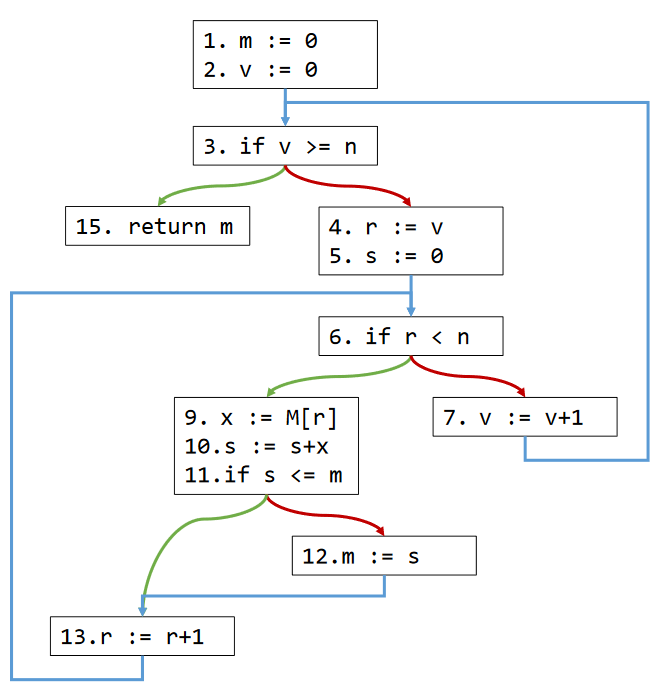
\includegraphics[width=\textwidth]{ex8_6p190}
\end{figure}

\section{Oefening 9.1 p217}
?
	\chapter{Oefeningensessie 3}


\section{Oefening 10.1 p223}

Gegeven het volgende programma:
\begin{lstlisting}

\end{lstlisting}
	\chapter{Oefeningensessie 4}


\section{Oefening Scheduling}

Gegeven de volgende machinecode:
\begin{lstlisting}
a	ld r1, [0x8000]
b	ld r2, [0x8004]
c	add r3, r1, 1
d	mul r4, r1, r2
e	sal r5, r2, 1
f	lea r6, [0x8000 + r4]
g	div r7, r5, r3
h	add r8, r6, r3
i	mul	r9, r4, r7
j	lea r10, [0x8000 + r5]
k	add r11, r9, r8
l	add r12, r9, r10
m	ld r13, [r12]
n	st [r11], r13
\end{lstlisting}
Veronderstel ook geen geheugenafhankelijkheden, en de volgende cycli:
\begin{table}
	\begin{tabular}{| l | l |}
		\hline 
		\textbf{Instructie} & \textbf{Cycli} \\
		\hline
		ld, st, mul & 2 \\
		div & 3 \\
		add, lea, sal & 1
	\end{tabular}
\end{table}

\begin{enumerate}
	\item Geef de data dependence graph.
	\item Schedule het basisblok op een 3-slot VLIW architectuur met 3 pipeline stages (OF, FU en WB) met operand forwarding.
	
\end{enumerate}

\section{Oefening 18.1 p431}
Gegeven de volgende flow graph

\begin{enumerate}
	\item Bepaal de dominators van elke node.
	\item Geef de immediate dominator tree.
	\item Identificeer de verzameling van nodes van elke natuurlijke lus.
\end{enumerate}

\section{Oefening Static Single Assignment}
Gegegeven het volgende programma:




\begin{enumerate}
	\item 
\end{enumerate}
\end{document}